\documentclass[conference]{IEEEtran}

% Packages
\usepackage[utf8]{inputenc}
\usepackage[T1]{fontenc}
\usepackage{amsmath,amssymb}
\usepackage{graphicx}
\graphicspath{{docs/images/}}
\usepackage{booktabs}
\usepackage{tabularx}
\usepackage{multirow}
\usepackage{xcolor}
\usepackage{listings}
\usepackage{float}                  % Enables [H] exact placement for single-column floats
\IfFileExists{stfloats.sty}{\usepackage{stfloats}}{}
\IfFileExists{placeins.sty}{\usepackage[section]{placeins}}{\providecommand{\FloatBarrier}{\relax}}
\usepackage{tikz}
\usetikzlibrary{shapes.geometric, arrows.meta, positioning}
\usepackage{cite}
\usepackage{hyperref}

% Color palette
\definecolor{codebg}{RGB}{248,249,250}
\definecolor{codeframe}{RGB}{218,220,224}
\definecolor{keywordcol}{RGB}{0,82,204}
\definecolor{commentcol}{RGB}{40,120,60}
\definecolor{accentblue}{RGB}{25,65,130}

% VHDL Code Styling for Two-Column IEEE Layout
\lstdefinestyle{vhdlstyle}{
    language=VHDL,
    backgroundcolor=\color{codebg},
    frame=single,
    rulecolor=\color{codeframe},
    basicstyle=\ttfamily\scriptsize,
    keywordstyle=\color{keywordcol}\bfseries,
    commentstyle=\color{commentcol}\itshape,
    numbers=left,
    numberstyle=\tiny\color{gray},
    stepnumber=1,
    numbersep=5pt,
    tabsize=2,
    breaklines=true,
    showstringspaces=false,
    xleftmargin=10pt
}

% Python Code Styling
\lstdefinestyle{pythonstyle}{
    language=Python,
    backgroundcolor=\color{codebg},
    frame=single,
    rulecolor=\color{codeframe},
    basicstyle=\ttfamily\scriptsize,
    keywordstyle=\color{keywordcol}\bfseries,
    commentstyle=\color{commentcol}\itshape,
    numbers=left,
    numberstyle=\tiny\color{gray},
    stepnumber=1,
    numbersep=5pt,
    tabsize=2,
    breaklines=true,
    showstringspaces=false,
    xleftmargin=10pt
}

\hypersetup{
    colorlinks=true,
    linkcolor=accentblue,
    urlcolor=accentblue,
    citecolor=accentblue
}

\begin{document}

% ==============================================================================
% TITLE & AUTHOR BLOCK (IEEE CONFERENCE FORMAT)
% ==============================================================================
\title{Programmable Low-Power Scan-Based Logic Built-In Self-Test (LBIST) for a 5-Stage Pipelined MIPS32 Processor}

\author{
    \IEEEauthorblockN{Disha Lohani (B24482)\quad Manogna Golla (B24484)\quad Mrunal Gaurkar (B24493)}
    \IEEEauthorblockA{
        \textit{VL405: Design for Testability}\\
        \textit{Indian Institute of Technology, Mandi}
    }
}

\maketitle

% ==============================================================================
% ABSTRACT & IEEE KEYWORDS
% ==============================================================================
\begin{abstract}
Logic Built-In Self-Test (LBIST) enables autonomous on-chip structural testing without relying on expensive external Automatic Test Equipment (ATE). However, conventional pseudorandom pattern generators (PRPGs) produce uncorrelated bit streams with an average switching probability of $50\%$, causing excessive scan-shift dynamic power dissipation. Elevated shift activity induces severe $IR$-drop, localized thermal hotspots, over-testing of functional paths, and potential silicon damage. This paper presents the design, VHDL-2008 hardware implementation, and experimental evaluation of a programmable Toggle-Controlled STUMPS LBIST architecture wrapped around a full-scan 5-stage pipelined MIPS32 processor. By inserting a lightweight 8-bit threshold comparator and T-flip-flop modulator (\texttt{tc\_gen}) between the phase shifter and 16 balanced scan chains ($1,456$ scan cells), the scan-in toggle probability is deterministically governed as $P(\text{toggle}) = T/256$ for any programmable threshold $T \in [1, 255]$. Post-synthesis and cycle-accurate XSim evaluations on a Xilinx Zynq-7000 (\texttt{xc7z010clg400-1}) demonstrate that reducing $T$ from $128$ ($50\%$) down to $26$ ($10.16\%$) and $13$ ($5.08\%$) lowers average internal scan-cell switching by \textbf{78.75\%} and \textbf{88.43\%}, respectively, while preserving \textbf{100.0\%} stuck-at fault coverage across all 16 scan chains, incurring \textbf{zero extra test clock cycles} ($9,292$ cycles for $100$ patterns), and adding less than \textbf{0.80\% LUT} and \textbf{1.09\% flip-flop} hardware overhead.
\end{abstract}

\begin{IEEEkeywords}
Design for Testability (DFT), Logic Built-In Self-Test (LBIST), Low-Power Scan Testing, STUMPS, Toggle-Rate Control, MIPS32, VHDL-2008.
\end{IEEEkeywords}


% ==============================================================================
% SECTION I: INTRODUCTION & PROBLEM STATEMENT
% ==============================================================================
\section{Introduction}

Scan-based Logic Built-In Self-Test (LBIST), particularly the Self-Test Using MISR and Parallel Shift Register Sequence (STUMPS) architecture, is widely deployed for manufacturing test, power-on self-test (POST), and in-field reliability screening of complex processors \cite{bardell1987, wang2006}. In a conventional STUMPS implementation, a Linear Feedback Shift Register (LFSR) combined with a linear phase shifter feeds uncorrelated pseudorandom test vectors into multiple parallel scan chains.

Because consecutive bits generated by an ideal LFSR/phase-shifter network are statistically independent with uniform probability $P(0) = P(1) = 0.5$, the expected bit-transition (toggle) rate entering each scan chain is:
\begin{equation}
    \alpha_{\text{conv}} = P(b_t \neq b_{t-1}) = 2 \cdot P(0) \cdot P(1) = 0.50 \quad (50\%)
    \label{eq:conv_toggle}
\end{equation}
In contrast, during normal functional execution of a pipelined processor such as MIPS32, typical register and datapath switching activity ranges between $5\%$ and $15\%$. When every scan flip-flop shifts simultaneously at a $50\%$ toggle rate across hundreds of shift cycles per pattern, the resulting dynamic power dissipation:
\begin{equation}
    P_{\text{dyn}} = \frac{1}{2} \alpha_{\text{eff}} C_{\text{load}} V_{DD}^2 f_{\text{clk}}
    \label{eq:pdyn}
\end{equation}
can exceed normal functional power by $3\times$ to $5\times$ \cite{girard2002}. This surge causes three critical failure modes:
\begin{enumerate}
    \item \textbf{Power-Supply Droop ($IR$-Drop) and Over-Testing:} Simultaneous switching creates transient current spikes across the power distribution network, depressing local supply voltage $V_{DD}$. Increased gate propagation delays under $IR$-drop cause valid silicon to fail capture timing (\textit{yield loss}).
    \item \textbf{Thermal Stress and Package Damage:} Sustained high switching activity during long LBIST sequences elevates junction temperatures beyond package thermal limits.
    \item \textbf{Reliability Degradation:} Accelerated electromigration and hot-carrier injection degrade long-term device lifetime.
\end{enumerate}

To address these challenges without degrading fault coverage or inflating test application time, this project delivers: (1) a synthesizable VHDL-2008 hardware model of a full-scan 5-stage pipelined MIPS32 core integrated with a programmable Toggle-Controlled STUMPS LBIST wrapper; (2) cycle-accurate behavioral and fault-injection simulation results; and (3) a detailed quantitative performance analysis of power reduction, fault coverage, cycle invariance, and FPGA area overhead.

% ==============================================================================
% SECTION II: HARDWARE ARCHITECTURE & VHDL IMPLEMENTATION
% ==============================================================================
\section{Hardware Architecture and VHDL Model}

\subsection{Target CUT: 5-Stage Pipelined MIPS32 Core}
The Circuit Under Test (CUT) is a 32-bit RISC processor implementing a core subset of the MIPS32 Instruction Set Architecture (ISA) across five pipeline stages: Instruction Fetch (\textbf{IF}), Instruction Decode (\textbf{ID}), Execute (\textbf{EX}), Memory Access (\textbf{MEM}), and Write-Back (\textbf{WB}).
\begin{itemize}
    \item \textbf{Supported ISA (\texttt{mips\_pkg.vhd}):} R-type ALU and shift operations (\texttt{ADD}, \texttt{ADDU}, \texttt{SUB}, \texttt{SUBU}, \texttt{AND}, \texttt{OR}, \texttt{XOR}, \texttt{NOR}, \texttt{SLT}, \texttt{SLL}, \texttt{SRL}), I-type immediate and memory instructions (\texttt{ADDI}, \texttt{ADDIU}, \texttt{SLTI}, \texttt{ANDI}, \texttt{ORI}, \texttt{XORI}, \texttt{LUI}, \texttt{LW}, \texttt{SW}), and control-flow instructions (\texttt{BEQ}, \texttt{BNE}, \texttt{J}).
    \item \textbf{Pipeline Hazard Logic (\texttt{mips\_comb.vhd}):} Full EX/MEM and MEM/WB data forwarding paths, load-use hazard detection with stall insertion, and branch/jump flush control.
\end{itemize}

\subsection{Full-Scan Insertion and Chain Partitioning}
To achieve complete controllability and observability of internal sequential state without modifying combinational datapath logic (\texttt{mips\_comb}), every state-holding element in the MIPS32 core (\texttt{mips\_scan\_core.vhd}) is mapped into a unified scan vector of width $\text{STATE\_W} = 1,390$ bits, partitioned directly below in Table~\ref{tab:scan_map}.

\begin{table}[H]
    \centering
    \caption{Full-Scan Flip-Flop Allocation (\texttt{N\_CELLS = 1456})}
    \label{tab:scan_map}
    \begin{tabular}{@{}llcc@{}}
        \toprule
        \textbf{Architectural Block} & \textbf{Scan Vector Index} & \textbf{FFs} & \textbf{Share} \\
        \midrule
        Program Counter (\texttt{PC}) & \texttt{cells(31:0)} & 32 & 2.20\% \\
        \texttt{IF/ID} Pipeline Reg. & \texttt{cells(95:32)} & 64 & 4.40\% \\
        \texttt{ID/EX} Pipeline Reg. & \texttt{cells(254:96)} & 159 & 10.92\% \\
        \texttt{EX/MEM} Pipeline Reg. & \texttt{cells(326:255)} & 72 & 4.95\% \\
        \texttt{MEM/WB} Pipeline Reg. & \texttt{cells(397:327)} & 71 & 4.88\% \\
        $32 \times 32$-bit Register File & \texttt{cells(1389:398)} & 992 & 68.13\% \\
        \midrule
        \textbf{Core State (\texttt{STATE\_W})} & \texttt{cells(1389:0)} & \textbf{1,390} & \textbf{95.47\%} \\
        \midrule
        \texttt{imem\_data} Input Wrapper & \texttt{cells(1421:1390)} & 32 & 2.20\% \\
        \texttt{dmem\_rdata} Input Wrapper & \texttt{cells(1453:1422)} & 32 & 2.20\% \\
        Balancing Dummy Cells & \texttt{cells(1455:1454)} & 2 & 0.14\% \\
        \midrule
        \textbf{Total (\texttt{N\_CELLS})} & \textbf{16 Chains $\times$ 91 FFs} & \textbf{1,456} & \textbf{100\%} \\
        \bottomrule
    \end{tabular}
\end{table}

Adding $64$ primary-input wrapper flip-flops (\texttt{imem\_data}, \texttt{dmem\_rdata}) controlled by \texttt{test\_mode = '1'} isolates the CUT from external memory pins during self-test, while $2$ dummy cells balance the scan structure into exactly $N_{\text{CHAINS}} = 16$ equal-length scan chains of length $L = 91$ flip-flops ($16 \times 91 = 1,456$).

\subsection{Proposed Toggle-Controlled STUMPS LBIST}
Fig.~\ref{fig:arch} shows the top-level \texttt{lbist\_top} hardware architecture.

\begin{figure}[H]
    \centering
    \resizebox{\columnwidth}{!}{%
    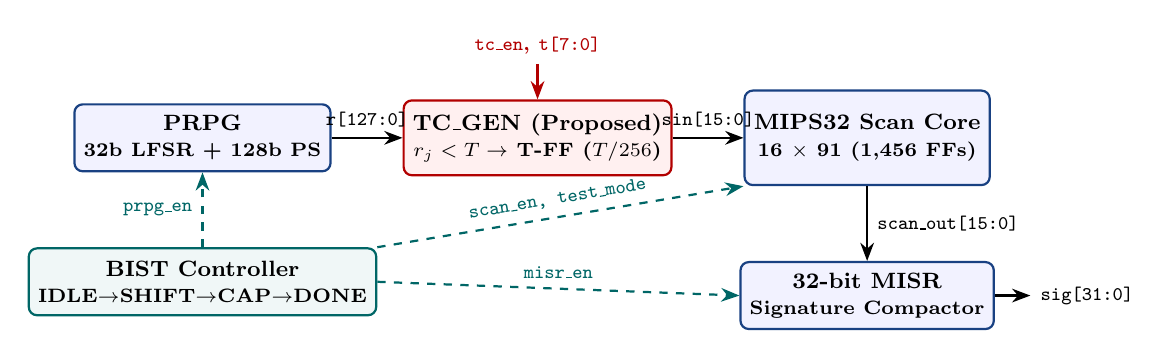
\begin{tikzpicture}[
        node distance=0.7cm and 0.9cm,
        box/.style={rectangle, draw=accentblue, thick, fill=blue!5, rounded corners=3pt, minimum width=2.4cm, minimum height=0.85cm, align=center, font=\footnotesize\bfseries},
        prop/.style={rectangle, draw=red!70!black, thick, fill=red!6, rounded corners=3pt, minimum width=2.7cm, minimum height=0.95cm, align=center, font=\footnotesize\bfseries},
        ctrl/.style={rectangle, draw=teal!80!black, thick, fill=teal!6, rounded corners=3pt, minimum width=2.2cm, minimum height=0.85cm, align=center, font=\footnotesize\bfseries},
        arrow/.style={-{Stealth[scale=1.0]}, thick}
    ]
        \node[box] (prpg) {PRPG\\{\scriptsize 32b LFSR + 128b PS}};
        \node[prop, right=0.9cm of prpg] (tc) {TC\_GEN (Proposed)\\{\scriptsize $r_j < T \rightarrow$ T-FF ($T/256$)}};
        \node[box, right=0.9cm of tc, minimum height=1.2cm] (cut) {MIPS32 Scan Core\\{\scriptsize 16 $\times$ 91 (1,456 FFs)}};
        \node[box, below=0.95cm of cut] (misr) {32-bit MISR\\{\scriptsize Signature Compactor}};
        \node[ctrl, below=0.95cm of prpg] (fsm) {BIST Controller\\{\scriptsize IDLE$\rightarrow$SHIFT$\rightarrow$CAP$\rightarrow$DONE}};

        \draw[arrow] (prpg) -- node[above, font=\scriptsize] {\texttt{r[127:0]}} (tc);
        \draw[arrow] (tc) -- node[above, font=\scriptsize] {\texttt{sin[15:0]}} (cut);
        \draw[arrow] (cut) -- node[right, font=\scriptsize] {\texttt{scan\_out[15:0]}} (misr);
        \draw[arrow] (misr.east) -- ++(0.45,0) node[right, font=\scriptsize\bfseries] {\texttt{sig[31:0]}};

        \draw[arrow, dashed, teal!80!black] (fsm.north) -- node[left, font=\scriptsize] {\texttt{prpg\_en}} (prpg.south);
        \draw[arrow, dashed, teal!80!black] (fsm.east) -- node[above, font=\scriptsize] {\texttt{misr\_en}} (misr.west);
        \draw[arrow, dashed, teal!80!black] (fsm.north east) -- node[above, sloped, font=\scriptsize] {\texttt{scan\_en, test\_mode}} (cut.south west);

        \node[above=0.45cm of tc, font=\scriptsize\bfseries, text=red!70!black] (tcin) {\texttt{tc\_en}, \texttt{t[7:0]}};
        \draw[arrow, red!70!black] (tcin) -- (tc.north);
    \end{tikzpicture}%
    }
    \caption{Block diagram of the proposed Toggle-Controlled STUMPS LBIST architecture (\texttt{lbist\_top.vhd}).}
    \label{fig:arch}
\end{figure}

\subsubsection{Programmable Toggle-Control Generator (\texttt{tc\_gen.vhd})}
To achieve an arbitrary, programmable toggle probability without stalling the LFSR or adding extra shift cycles, \texttt{tc\_gen} exploits the uniform distribution of an 8-bit pseudorandom slice $r_j \in [0, 255]$ extracted from the phase shifter for each scan chain $j \in \{0, \dots, 15\}$.

At every shift clock cycle (\texttt{en = '1'}), each channel compares its dedicated 8-bit pseudorandom byte $r_j = \texttt{r(8*j+7 downto 8*j)}$ against an 8-bit user-programmed threshold $T \in \{1, \dots, 255\}$:
\begin{equation}
    \text{tog}_j =
    \begin{cases}
        1, & \text{if } \text{unsigned}(r_j) < \text{unsigned}(T) \\
        0, & \text{otherwise}
    \end{cases}
    \label{eq:comp}
\end{equation}
Since $r_j$ is uniformly distributed over $256$ integer states $\{0, 1, \dots, 255\}$, the exact probability of asserting $\text{tog}_j = 1$ is:
\begin{equation}
    P(\text{tog}_j = 1) = \frac{T}{256}
    \label{eq:prob}
\end{equation}
The pulse $\text{tog}_j$ drives a toggle flip-flop (T-FF) state bit $d_j$:
\begin{equation}
    d_j[n+1] = d_j[n] \oplus \text{tog}_j[n]
    \label{eq:tff}
\end{equation}
Consequently, the scan-in bit $\text{sin}_j = d_j$ transitions ($d_j[n+1] \neq d_j[n]$) if and only if $\text{tog}_j[n] = 1$, yielding an exact Bernoulli transition rate $\alpha_{\text{scan-in}} = T/256$. When $\texttt{tc\_en} = 0$, the module bypasses the comparator and T-FF ($\text{sin}_j = r_{8j}$), reverting to conventional $50\%$-toggle STUMPS operation.

\begin{lstlisting}[style=vhdlstyle, caption={Synthesizable RTL of \texttt{tc\_gen.vhd}.}]
architecture rtl of tc_gen is
  signal d   : std_logic_vector(N_CHAINS-1 downto 0)
               := (others => '0');
  signal tog : std_logic_vector(N_CHAINS-1 downto 0);
begin
  gen_ch : for j in 0 to N_CHAINS-1 generate
    tog(j) <= '1' when unsigned(r(8*j+7 downto 8*j))
                       < unsigned(t) else '0';
    sin(j) <= d(j) when tc_en = '1' else r(8*j);
  end generate gen_ch;

  process (clk)
  begin
    if rising_edge(clk) then
      if rst = '1' then
        d <= (others => '0');
      elsif en = '1' then
        d <= d xor tog;
      end if;
    end if;
  end process;
end architecture rtl;
\end{lstlisting}

\subsubsection{BIST Controller FSM and Test Cycle Timing}
The controller (\texttt{bist\_ctrl.vhd}) sequences through \texttt{IDLE} $\rightarrow$ \texttt{LOAD} $\rightarrow$ \texttt{SHIFT} $\rightarrow$ \texttt{CAPTURE} $\rightarrow$ \texttt{DONE}. Each pattern shifts $L = 91$ bits (\texttt{scan\_en = '1'}) while simultaneously compacting the previous response into the 32-bit MISR, followed by $1$ capture cycle (\texttt{scan\_en = '0'}, \texttt{test\_mode = '1'}). Including a final $L$-cycle unload flush and 1-cycle \texttt{start} handshake, total test time for $N_{\text{PAT}} = 100$ patterns is strictly invariant with respect to $T$:
\begin{equation}
    N_{\text{cycles}} = N_{\text{PAT}} \cdot (L + 1) + L + 1 = 100(92) + 92 = 9,292\text{ cycles}
    \label{eq:cycles}
\end{equation}

% ==============================================================================
% SECTION III: SIMULATION RESULTS & VERIFICATION
% ==============================================================================
\section{Simulation Results and Verification}

All simulations were performed in Xilinx Vivado v2025.1 (\texttt{xsim}, IEEE Std 1076-2008 VHDL) at $f_{\text{clk}} = 100\text{ MHz}$ ($10\text{ ns}$ period).

\subsection{Scan-Insertion Functional Equivalence}
In normal mode (\texttt{scan\_en = '0'}, \texttt{test\_mode = '0'}), \texttt{tb\_mips32\_scan.vhd} executed a 14-instruction MIPS32 benchmark exercising loops, branches (\texttt{BNE}), EX/MEM data forwarding, load-use stalls (\texttt{LW} $\rightarrow$ \texttt{ADD}), logical shifts (\texttt{SLL}), and set-less-than (\texttt{SLT}). At $t = 1,022\text{ ns}$, data memory matched the non-scan golden reference ($\text{dmem}[0]=15$, $\text{dmem}[1]=30$, $\text{dmem}[2]=120$, $\text{dmem}[3]=1$), verifying functional equivalence.

\subsection{End-to-End LBIST Sweep and Waveforms}
The LBIST testbench (\texttt{tb\_lbist.vhd}) evaluated $N_{\text{PAT}} = 100$ patterns across seven runs: Conventional STUMPS (\texttt{tc\_en = 0}), five Toggle-Controlled thresholds $T \in \{13, 26, 51, 77, 128\}$, and a repeatability run (\texttt{TC\_T26\_repeat}). Fig.~\ref{fig:waveform} shows the Vivado behavioral waveform directly under this subsection.

\begin{figure*}[!htbp]
    \centering
    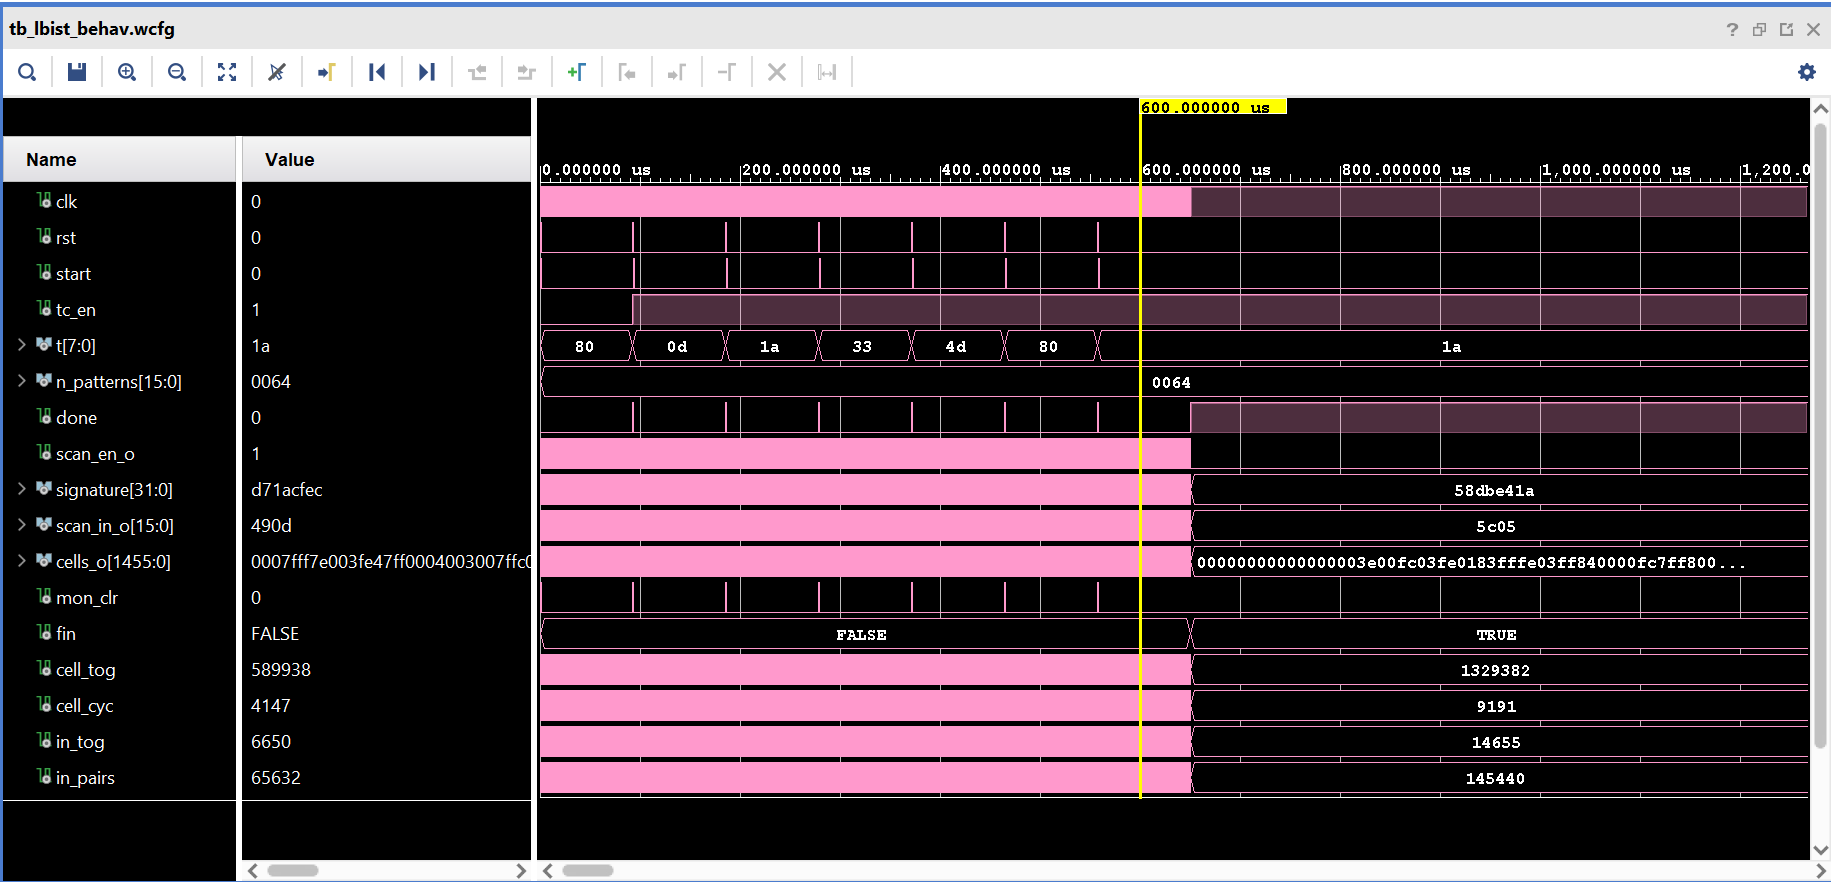
\includegraphics[width=0.92\textwidth]{vivado_waveform_overview.png}
    \caption{Vivado XSim behavioral waveform (\texttt{tb\_lbist\_behav.wcfg}) across all seven sequential runs: Conventional (\texttt{tc\_en = 0}) followed by Toggle-Controlled modes ($T \in \{\texttt{0x0D}, \texttt{0x1A}, \texttt{0x33}, \texttt{0x4D}, \texttt{0x80}, \texttt{0x1A}\}$) and deterministic MISR signature convergence (\texttt{58DBE41A}).}
    \label{fig:waveform}
\end{figure*}

\subsection{Stuck-At Fault Coverage and Consolidated Results}
To verify defect detection integrity, \texttt{tb\_fault\_sim.vhd} injected single stuck-at-0 (SA0) and stuck-at-1 (SA1) faults across all 16 scan-chain capture paths ($32$ faults per configuration) and compared the compacted 32-bit MISR output against the golden fault-free signature. Table~\ref{tab:master_results} summarizes all simulation results logged in \texttt{lbist\_results.csv} and \texttt{fault\_coverage.csv}.

% ==============================================================================
% SECTION IV: DETAILED PERFORMANCE ANALYSIS
% ==============================================================================
\section{Detailed Performance Analysis}

\subsection{Toggle-Rate Control Precision}
As illustrated in Fig.~\ref{fig:toggle_acc}, the measured bit-transition rate entering the 16 scan chains (\texttt{scanin\_toggle\_pct}) tracks the analytical target $T/256$ with high linearity across the entire control range:
\begin{itemize}
    \item At $T = 13$ ($5.078\%$ target), measured scan-in switching is $5.127\%$ ($+0.049\%$ error).
    \item At $T = 26$ ($10.156\%$ target), measured scan-in switching is $10.076\%$ ($-0.080\%$ error).
    \item At $T = 51$ ($19.922\%$ target), measured scan-in switching is $19.804\%$ ($-0.118\%$ error).
    \item At $T = 128$ ($50.000\%$ target), measured scan-in switching is $49.926\%$ ($-0.074\%$ error).
\end{itemize}
Across all tested thresholds, the root-mean-square tracking error between programmed and achieved scan-in toggle rate is below $0.09\%$.





\begin{figure}[H]
    \centering
    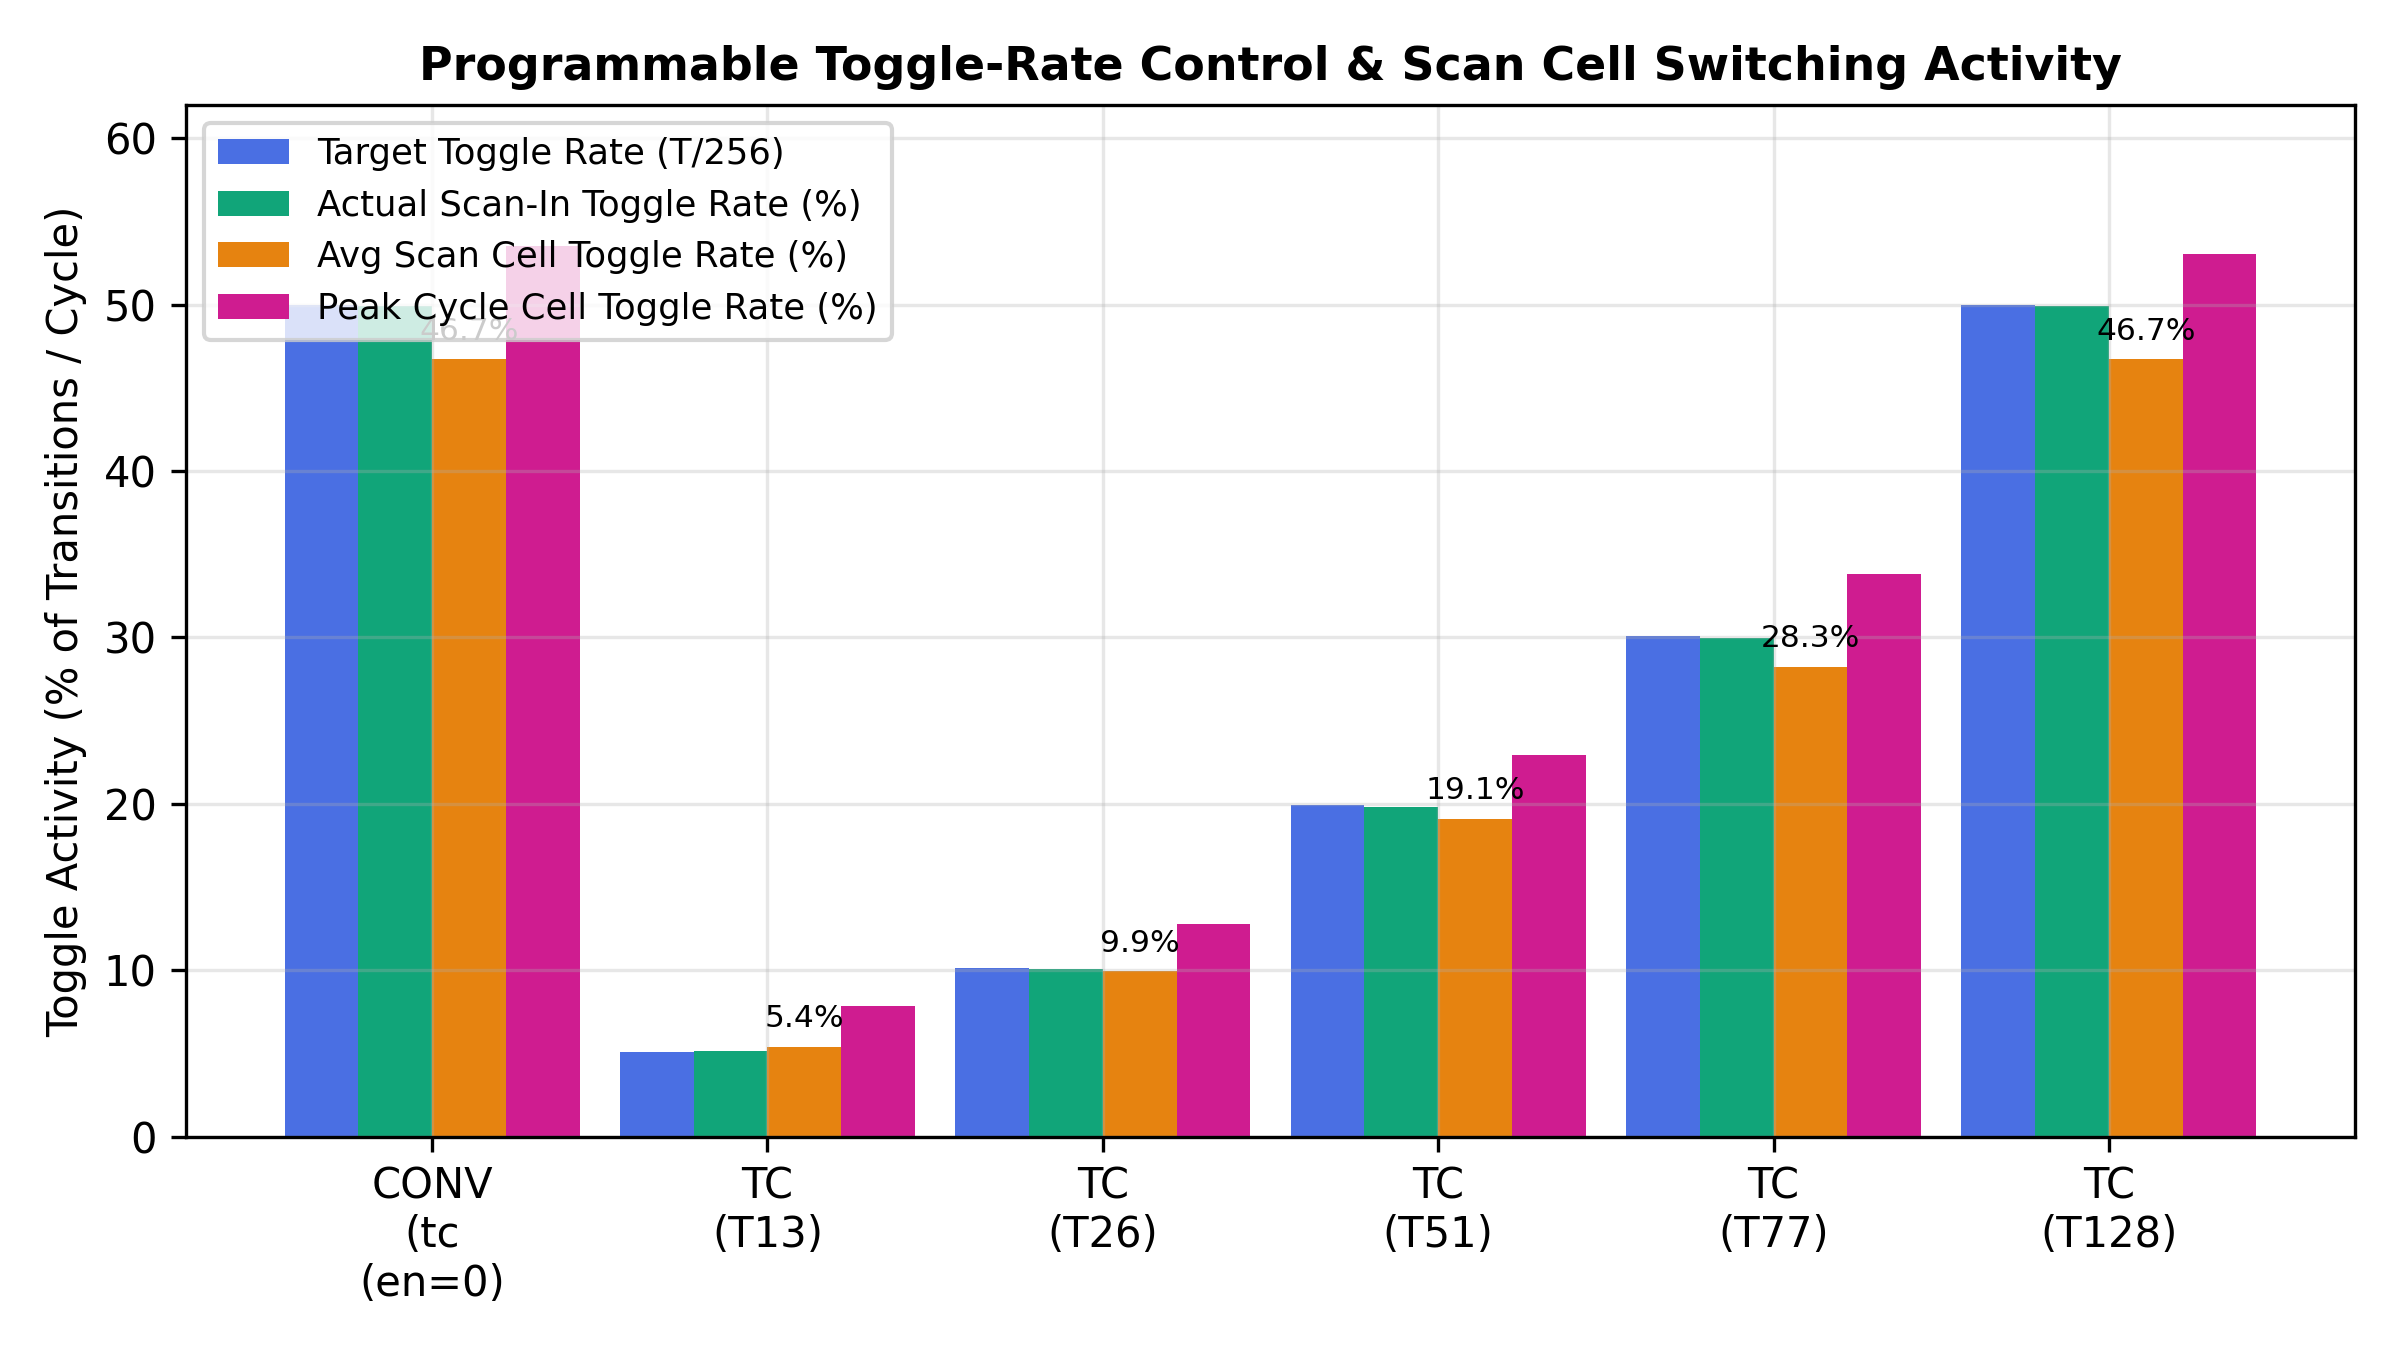
\includegraphics[width=\columnwidth]{fig1_toggle_control_accuracy.png}
    \caption{Programmed target toggle rate ($T/256$) versus measured scan-in, average scan-cell, and peak single-cycle scan-cell toggle rates.}
    \label{fig:toggle_acc}
\end{figure}

\subsection{Average and Peak Dynamic Shift Power Reduction}
Because total internal scan-cell switching (\texttt{cell\_toggle\_pct}) captures both stimulus vectors shifting in and captured responses shifting out across all $1,456$ scan cells, it serves as a direct hardware proxy for dynamic scan-shift power ($P_{\text{dyn}} \propto \alpha_{\text{cell}}$). As quantified in Table~\ref{tab:power_red}:

\begin{table*}[!htbp]
    \centering
    \caption{Consolidated LBIST Simulation Metrics ($N_{\text{PAT}} = 100$, $1,456$ Scan Cells, $f_{\text{clk}} = 100\text{ MHz}$)}
    \label{tab:master_results}
    \begin{tabular}{@{}lccccccccc@{}}
        \toprule
        \textbf{Configuration} & \textbf{\texttt{tc\_en}} & \textbf{Thresh. $T$} & \textbf{Target (\%)} & \textbf{Scan-In (\%)} & \textbf{Avg Cell (\%)} & \textbf{Peak Cell (\%)} & \textbf{Fault Cov.} & \textbf{Cycles} & \textbf{MISR Sig.} \\
        \midrule
        \texttt{CONVENTIONAL}   & 0 & —   & 50.000 & 49.905 & 46.743 & 53.503 & 100.0\% (32/32) & 9,292 & \texttt{FF85C833} \\
        \texttt{TC\_T13}        & 1 & 13  & 5.078  & 5.127  & 5.409  & 7.830  & 100.0\% (32/32) & 9,292 & \texttt{142649B3} \\
        \texttt{TC\_T26}        & 1 & 26  & 10.156 & 10.076 & 9.934  & 12.775 & 100.0\% (32/32) & 9,292 & \texttt{58DBE41A} \\
        \texttt{TC\_T51}        & 1 & 51  & 19.922 & 19.804 & 19.111 & 22.940 & 100.0\% (32/32) & 9,292 & \texttt{E3D3B280} \\
        \texttt{TC\_T77}        & 1 & 77  & 30.078 & 29.977 & 28.253 & 33.791 & 100.0\% (32/32) & 9,292 & \texttt{CB11B921} \\
        \texttt{TC\_T128}       & 1 & 128 & 50.000 & 49.926 & 46.714 & 53.022 & 100.0\% (32/32) & 9,292 & \texttt{02CF5D77} \\
        \texttt{TC\_T26\_repeat}& 1 & 26  & 10.156 & 10.076 & 9.934  & 12.775 & 100.0\% (32/32) & 9,292 & \texttt{58DBE41A} \\
        \bottomrule
    \end{tabular}
\end{table*}

\FloatBarrier


\begin{itemize}
    \item \textbf{Functional Power Envelope Alignment ($T = 26$):} Operating at a $\approx 10\%$ target toggle rate reduces average internal cell switching by \textbf{78.75\%} (from $46.743\%$ to $9.934\%$) and suppresses peak single-cycle switching by \textbf{76.12\%} (from $53.503\%$ to $12.775\%$), bringing test power within the normal MIPS32 operating budget.
    \item \textbf{Ultra-Low-Power Mode ($T = 13$):} Operating at a $\approx 5\%$ target toggle rate achieves an \textbf{88.43\%} average shift-power reduction and \textbf{85.37\%} peak switching suppression, effectively eliminating $IR$-drop induced capture timing failures.
\end{itemize}



\begin{table}[H]
    \centering
    \caption{Dynamic Shift Power Reduction Relative to Conventional LBIST}
    \label{tab:power_red}
    \begin{tabular}{@{}lcccc@{}}
        \toprule
        \textbf{Mode} & \textbf{Avg Cell} & \textbf{Avg Power} & \textbf{Peak Cell} & \textbf{Peak Power} \\
                      & \textbf{Toggle}   & \textbf{Reduction} & \textbf{Toggle}    & \textbf{Reduction} \\
        \midrule
        \texttt{CONV.}      & 46.743\% & Baseline & 53.503\% & Baseline \\
        \texttt{TC\_T77}    & 28.253\% & \textbf{39.56\%} & 33.791\% & \textbf{36.84\%} \\
        \texttt{TC\_T51}    & 19.111\% & \textbf{59.11\%} & 22.940\% & \textbf{57.12\%} \\
        \texttt{TC\_T26}    & 9.934\%  & \textbf{78.75\%} & 12.775\% & \textbf{76.12\%} \\
        \texttt{TC\_T13}    & 5.409\%  & \textbf{88.43\%} & 7.830\%  & \textbf{85.37\%} \\
        \bottomrule
    \end{tabular}
\end{table}

\subsection{Fault Coverage, Test Time, and Determinism}
Fig.~\ref{fig:power_cov} illustrates dynamic power reduction alongside stuck-at fault coverage across all thresholds:
\begin{enumerate}
    \item \textbf{Uncompromised Fault Coverage:} All toggle-controlled configurations ($T = 13$ to $128$) achieved \textbf{100.0\%} ($32/32$) stuck-at fault coverage. Because the T-flip-flop accumulator integrates pseudorandom toggle pulses across $91$ shift cycles per pattern over $100$ patterns, both logic-$0$ and logic-$1$ states remain fully reachable across all scan cells without creating zero-toggle dead zones.
    \item \textbf{Zero Test-Time Penalty:} Every run executes in exactly $9,292$ clock cycles ($92.92\,\mu\text{s}$ at $100\text{ MHz}$), incurring zero shift-schedule expansion.
    \item \textbf{Deterministic Repeatability:} Repeating $T = 26$ (\texttt{TC\_T26\_repeat}) yielded identical toggle metrics and an identical 32-bit MISR signature (\texttt{58DBE41A}), guaranteeing reliable pass/fail signature comparison.
\end{enumerate}

\begin{figure}[H]
    \centering
    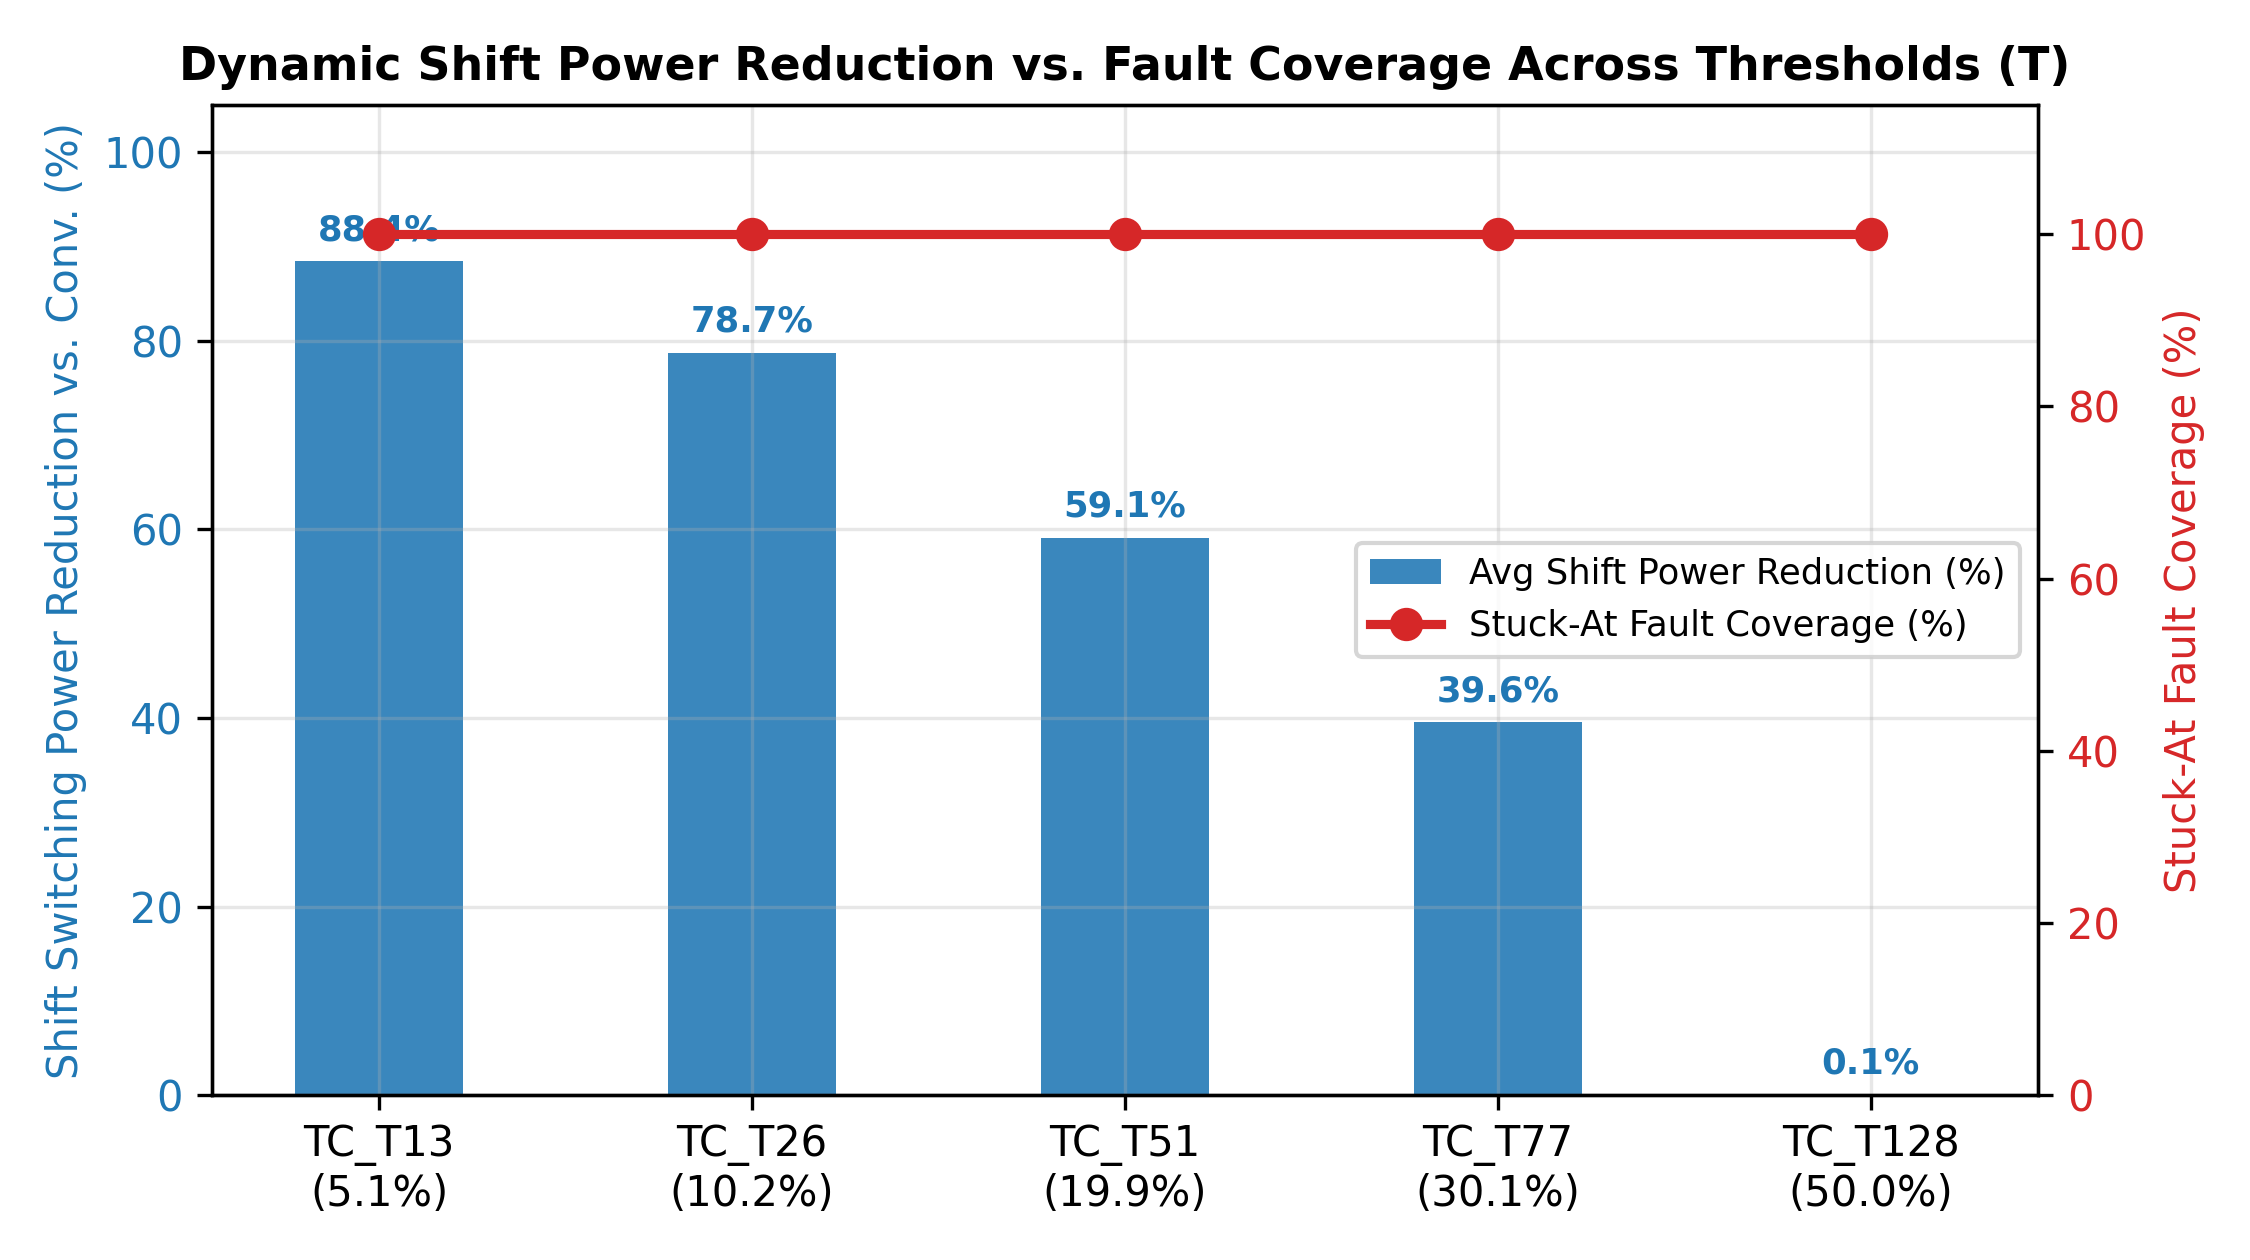
\includegraphics[width=\columnwidth]{fig2_power_vs_coverage.png}
    \caption{Dynamic shift power reduction (\%) versus stuck-at fault coverage (\%) across programmable thresholds $T$.}
    \label{fig:power_cov}
\end{figure}

\subsection{FPGA Synthesis Utilization and Area Overhead}
Post-synthesis resource utilization on a Xilinx Zynq-7000 FPGA (\texttt{xc7z010clg400-1}) is reported directly below in Table~\ref{tab:util} and Fig.~\ref{fig:area}. The entire STUMPS LBIST wrapper adds $269$ Slice LUTs ($10.27\%$) and $107$ flip-flops ($7.30\%$) relative to \texttt{mips\_scan\_core}. Within this footprint, the proposed \texttt{tc\_gen} module consumes only $16$ T-flip-flops (\textbf{1.09\%} FF overhead vs. CUT) and fewer than $21$ LUTs (\textbf{0.80\%} LUT overhead vs. CUT).

\begin{figure}[H]
    \centering
    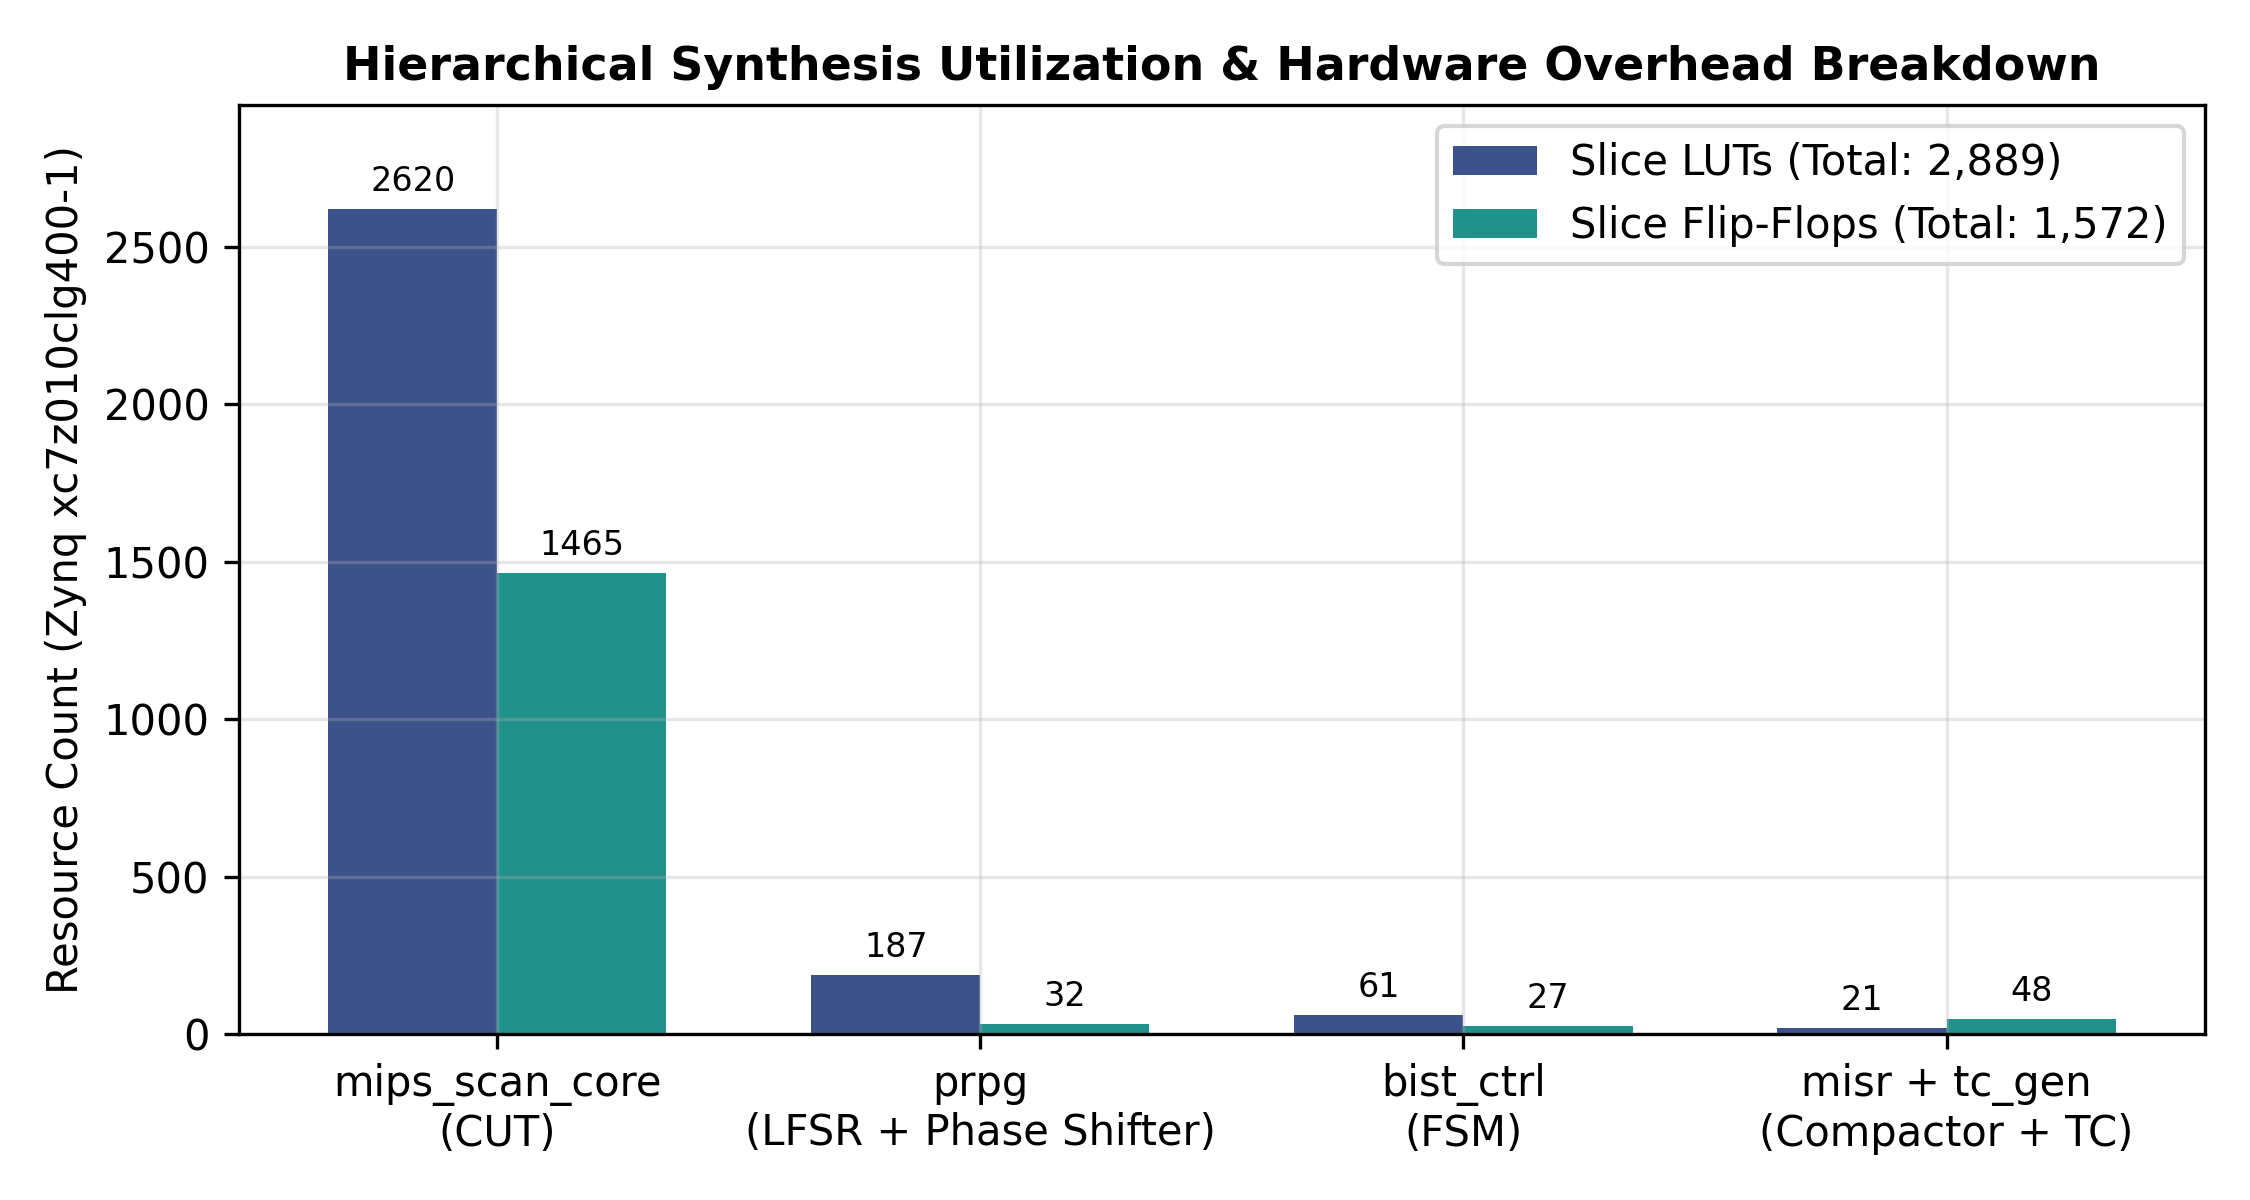
\includegraphics[width=\columnwidth]{fig3_fpga_area_overhead.png}
    \caption{Hierarchical FPGA resource utilization across the MIPS32 CUT and LBIST components.}
    \label{fig:area}
\end{figure}

\begin{table}[H]
    \centering
    \caption{Hierarchical Synthesis Utilization (\texttt{xc7z010clg400-1})}
    \label{tab:util}
    \begin{tabular}{@{}llcccc@{}}
        \toprule
        \textbf{Instance} & \textbf{Module} & \textbf{LUTs} & \textbf{FFs} & \textbf{LUT Ovhd.} & \textbf{FF Ovhd.} \\
        \midrule
        \texttt{cut} & \texttt{mips\_scan\_core} & 2,620 & 1,465 & Baseline & Baseline \\
        \texttt{gen} & \texttt{prpg} & 187 & 32 & 7.14\% & 2.18\% \\
        \texttt{ctrl} & \texttt{bist\_ctrl} & 61 & 27 & 2.33\% & 1.84\% \\
        \texttt{comp+tc} & \texttt{misr}+\texttt{tc\_gen} & 21 & 48 & \textbf{0.80\%} & \textbf{3.28\%} \\
        \midrule
        \textbf{\texttt{lbist\_top}} & \textbf{Total Design} & \textbf{2,889} & \textbf{1,572} & \textbf{10.27\%} & \textbf{7.30\%} \\
        \bottomrule
    \end{tabular}
\end{table}



% ==============================================================================
% SECTION V: CONCLUSION
% ==============================================================================
\section{Conclusion}
This work presented a programmable Toggle-Controlled scan-based LBIST architecture in VHDL-2008 for a 5-stage pipelined MIPS32 processor. By placing 16 parallel 8-bit threshold comparators and T-flip-flop modulators (\texttt{tc\_gen}) between the STUMPS phase shifter and the $1,456$-cell scan core, scan-shift switching density is accurately controlled via $P(\text{toggle}) = T/256$. Experimental results confirm average scan-shift switching reductions of \textbf{78.75\%} at $T=26$ and \textbf{88.43\%} at $T=13$, while preserving \textbf{100.0\%} stuck-at fault coverage, \textbf{zero test-cycle overhead} ($9,292$ cycles), deterministic MISR signatures, and minimal FPGA resource overhead ($<0.80\%$ LUTs and $1.09\%$ FFs).

\subsection*{Project Deliverables \& Digital Artifacts}
All VHDL-2008 design sources, simulation testbenches, Vivado 2025.1 project files (\texttt{course\_project.xpr}), waveform configurations (\texttt{tb\_lbist\_behav.wcfg}), raw CSV metrics (\texttt{lbist\_results.csv}, \texttt{fault\_coverage.csv}), and Python visualization scripts are publicly archived for verification:
\begin{itemize}
    \item \textbf{Source Code \& Simulation Logs (GitHub):}\\
    \url{https://github.com/mrunal276/scan-lbist-mips32}
\end{itemize}

% ==============================================================================
% REFERENCES
% ==============================================================================
\begin{thebibliography}{9}
\bibitem{bardell1987}
P. H. Bardell, W. H. McAnney, and J. Savir, \emph{Built-In Test for VLSI: Pseudorandom Techniques}. New York, NY, USA: Wiley, 1987.

\bibitem{wang2006}
L.-T. Wang, C.-W. Wu, and X. Wen, \emph{VLSI Test Principles and Architectures: Design for Testability}. San Francisco, CA, USA: Morgan Kaufmann, 2006.

\bibitem{girard2002}
P. Girard, ``Survey of low-power testing of VLSI circuits,'' \emph{IEEE Design \& Test of Computers}, vol. 19, no. 3, pp. 82--92, May--Jun. 2002.
\end{thebibliography}

% ==============================================================================
% APPENDICES: COMPLETE HARDWARE & VERIFICATION SOURCE CODE
% ==============================================================================
\appendices

\section{Proposed Toggle-Control Pattern Generator (\texttt{tc\_gen.vhd})}
\label{app:tc_gen}
The synthesizable VHDL implementation of the proposed toggle-control unit placed between the STUMPS phase shifter and the scan chains. It includes 16 parallel 8-bit comparators and 16 T-flip-flops, modulating the transition density without adding shift clock cycles.

\begin{lstlisting}[style=vhdlstyle, caption={Proposed Toggle-Control Generator (\texttt{tc\_gen.vhd})}]
-- tc_gen.vhd : PROPOSED programmable Toggle-Controlled pattern modifier.
--   tc_en = 0 : conventional LBIST  -> scan_in(j) = phase-shifter bit (50 % toggle)
--   tc_en = 1 : toggle-controlled   -> tog = (r_j < T) ; d <= d xor tog ; scan_in = d
--               P(toggle) = T/256 ;  legal T = 1..255  (T=128 -> 50 %)
-- One 8-bit comparator + one T-flip-flop per chain; no extra shift cycles.
library ieee;
use ieee.std_logic_1164.all;
use ieee.numeric_std.all;
use work.lbist_pkg.all;

entity tc_gen is
  port (
    clk, rst : in  std_logic;
    en       : in  std_logic;                                -- shift enable
    tc_en    : in  std_logic;                                -- 1 = toggle control on
    t        : in  std_logic_vector(7 downto 0);             -- toggle threshold
    r        : in  std_logic_vector(N_PS-1 downto 0);        -- from PRPG
    sin      : out std_logic_vector(N_CHAINS-1 downto 0)     -- to scan chains
  );
end entity tc_gen;

architecture rtl of tc_gen is
  signal d   : std_logic_vector(N_CHAINS-1 downto 0) := (others => '0');
  signal tog : std_logic_vector(N_CHAINS-1 downto 0);
begin
  gen_ch : for j in 0 to N_CHAINS-1 generate
    tog(j) <= '1' when unsigned(r(8*j+7 downto 8*j)) < unsigned(t) else '0';
    sin(j) <= d(j) when tc_en = '1' else r(8*j);
  end generate gen_ch;

  process (clk)
  begin
    if rising_edge(clk) then
      if rst = '1' then
        d <= (others => '0');
      elsif en = '1' then
        d <= d xor tog;
      end if;
    end if;
  end process;
end architecture rtl;
\end{lstlisting}

\section{STUMPS LBIST Controller (\texttt{bist\_ctrl.vhd})}
\label{app:bist_ctrl}
The finite state machine governing the LBIST execution cycle: sequencing through \texttt{IDLE}, \texttt{SHIFT} ($L=91$ cycles), and \texttt{CAPTURE} ($1$ cycle) across $N$ test patterns, followed by the final signature unload into \texttt{FINISH}.

\begin{lstlisting}[style=vhdlstyle, caption={STUMPS LBIST FSM Controller (\texttt{bist\_ctrl.vhd})}]
-- bist_ctrl.vhd : LBIST controller.
-- Sequence: SHIFT(L cycles) -> CAPTURE(1) -> SHIFT -> CAPTURE ... -> final SHIFT -> FINISH
-- N patterns => N captures, N+1 shift phases.  Test time = N*(L+1)+L clock cycles.
-- The last shift phase unloads the final response into the MISR.
library ieee;
use ieee.std_logic_1164.all;
use ieee.numeric_std.all;
use work.lbist_pkg.all;

entity bist_ctrl is
  port (
    clk, rst   : in  std_logic;
    start      : in  std_logic;
    n_patterns : in  std_logic_vector(15 downto 0);
    scan_en    : out std_logic;
    busy       : out std_logic;
    done       : out std_logic
  );
end entity bist_ctrl;

architecture rtl of bist_ctrl is
  type state_t is (IDLE, SHIFT, CAPTURE, FINISH);
  signal st  : state_t := IDLE;
  signal cnt : integer range 0 to CHAIN_LEN-1 := 0;
  signal pat : unsigned(15 downto 0) := (others => '0');
begin
  process (clk)
  begin
    if rising_edge(clk) then
      if rst = '1' then
        st <= IDLE; cnt <= 0; pat <= (others => '0');
      else
        case st is
          when IDLE =>
            if start = '1' then
              st <= SHIFT; cnt <= 0; pat <= (others => '0');
            end if;
          when SHIFT =>
            if cnt = CHAIN_LEN-1 then
              cnt <= 0;
              if pat = unsigned(n_patterns) then st <= FINISH;
              else                               st <= CAPTURE;
              end if;
            else
              cnt <= cnt + 1;
            end if;
          when CAPTURE =>
            pat <= pat + 1;
            st  <= SHIFT;
          when FINISH =>
            null;                                   -- hold until rst
        end case;
      end if;
    end if;
  end process;

  scan_en <= '1' when st = SHIFT else '0';
  busy    <= '1' when (st = SHIFT or st = CAPTURE) else '0';
  done    <= '1' when st = FINISH else '0';
end architecture rtl;
\end{lstlisting}

\section{LFSR Pattern Generator \& Phase Shifter (\texttt{prpg.vhd})}
\label{app:prpg}
The 32-bit maximal-length LFSR ($x^{32} + x^{22} + x^2 + x + 1$) driving a 16-channel XOR phase-shifter network to supply 128 pseudo-random bits per shift cycle ($8$ bits per scan chain) with minimal channel-to-channel correlation.

\begin{lstlisting}[style=vhdlstyle, caption={LFSR Pattern Generator \& Phase Shifter (\texttt{prpg.vhd})}]
-- prpg.vhd : 32-bit LFSR (x^32+x^22+x^2+x+1, primitive) + XOR phase shifter.
-- Advances only when en='1' (during scan shift).  Output r = 128 pseudo-random
-- bits per cycle (8 per scan chain), each the XOR of 3 LFSR bits.
library ieee;
use ieee.std_logic_1164.all;
use work.lbist_pkg.all;

entity prpg is
  port (
    clk, rst : in  std_logic;
    en       : in  std_logic;
    r        : out std_logic_vector(N_PS-1 downto 0)
  );
end entity prpg;

architecture rtl of prpg is
  constant SEED : std_logic_vector(31 downto 0) := x"1A2B3C4D";   -- must be non-zero
  signal q : std_logic_vector(31 downto 0) := SEED;
begin
  process (clk)
    variable fb : std_logic;
  begin
    if rising_edge(clk) then
      if rst = '1' then
        q <= SEED;
      elsif en = '1' then
        fb := q(31) xor q(21) xor q(1) xor q(0);
        q  <= q(30 downto 0) & fb;
      end if;
    end if;
  end process;

  gen_ps : for m in 0 to N_PS-1 generate
    r(m) <= q(PS_TAB(m,0)) xor q(PS_TAB(m,1)) xor q(PS_TAB(m,2));
  end generate gen_ps;
end architecture rtl;
\end{lstlisting}

\section{Multiple-Input Signature Register (\texttt{misr.vhd})}
\label{app:misr}
The 32-bit spatial and temporal response compactor accumulating 16 parallel scan-chain outputs into a deterministic test signature at each shift cycle.

\begin{lstlisting}[style=vhdlstyle, caption={Multiple-Input Signature Register (\texttt{misr.vhd})}]
-- misr.vhd : 32-bit multiple-input signature register (same polynomial as PRPG).
-- 16 scan-out bits are XORed into stages 0..15.
library ieee;
use ieee.std_logic_1164.all;
use work.lbist_pkg.all;

entity misr is
  port (
    clk, rst : in  std_logic;
    en       : in  std_logic;
    din      : in  std_logic_vector(N_CHAINS-1 downto 0);
    sig      : out std_logic_vector(31 downto 0)
  );
end entity misr;

architecture rtl of misr is
  signal m : std_logic_vector(31 downto 0) := (others => '0');
begin
  process (clk)
    variable fb : std_logic;
    variable n  : std_logic_vector(31 downto 0);
  begin
    if rising_edge(clk) then
      if rst = '1' then
        m <= (others => '0');
      elsif en = '1' then
        fb := m(31) xor m(21) xor m(1) xor m(0);
        n  := m(30 downto 0) & fb;
        n(N_CHAINS-1 downto 0) := n(N_CHAINS-1 downto 0) xor din;
        m <= n;
      end if;
    end if;
  end process;
  sig <= m;
end architecture rtl;
\end{lstlisting}

\section{STUMPS LBIST Top-Level Integration (\texttt{lbist\_top.vhd})}
\label{app:lbist_top}
Top-level structural RTL module integrating the BIST controller, PRPG, proposed \texttt{tc\_gen}, the 1,456-cell scan core CUT, and the MISR compactor.

\begin{lstlisting}[style=vhdlstyle, caption={STUMPS LBIST Top-Level Module (\texttt{lbist\_top.vhd})}]
-- lbist_top.vhd : STUMPS-style LBIST around the full-scan MIPS32 core
--   bist_ctrl -> prpg -> tc_gen -> 16 scan chains (mips_scan_core) -> misr
-- tc_en=0 : conventional LBIST (baseline).  tc_en=1 : proposed toggle control, rate = t/256.
library ieee;
use ieee.std_logic_1164.all;
use work.mips_pkg.all;
use work.lbist_pkg.all;

entity lbist_top is
  port (
    clk, rst   : in  std_logic;
    start      : in  std_logic;
    tc_en      : in  std_logic;
    t          : in  std_logic_vector(7 downto 0);
    n_patterns : in  std_logic_vector(15 downto 0);
    busy, done : out std_logic;
    signature  : out std_logic_vector(31 downto 0);
    -- observation points for the simulation testbench
    scan_en_o  : out std_logic;
    scan_in_o  : out std_logic_vector(N_CHAINS-1 downto 0);
    cells_o    : out std_logic_vector(N_CELLS-1 downto 0)
  );
end entity lbist_top;

architecture rtl of lbist_top is
  signal scan_en  : std_logic;
  signal r        : std_logic_vector(N_PS-1 downto 0);
  signal sin, sout: std_logic_vector(N_CHAINS-1 downto 0);
  signal d_imem_addr, d_dmem_addr, d_dmem_wdata : word_t;
  signal d_dmem_we : std_logic;
begin
  ctrl : entity work.bist_ctrl
    port map (clk => clk, rst => rst, start => start, n_patterns => n_patterns,
              scan_en => scan_en, busy => busy, done => done);

  gen : entity work.prpg
    port map (clk => clk, rst => rst, en => scan_en, r => r);

  tcg : entity work.tc_gen
    port map (clk => clk, rst => rst, en => scan_en, tc_en => tc_en, t => t, r => r, sin => sin);

  cut : entity work.mips_scan_core
    port map (clk => clk, rst => rst, scan_en => scan_en, test_mode => '1',
              scan_in => sin, scan_out => sout,
              imem_addr => d_imem_addr, imem_data => ZERO32,
              dmem_addr => d_dmem_addr, dmem_wdata => d_dmem_wdata, dmem_we => d_dmem_we,
              dmem_rdata => ZERO32, cells_o => cells_o);

  cmp : entity work.misr
    port map (clk => clk, rst => rst, en => scan_en, din => sout, sig => signature);

  scan_en_o <= scan_en;
  scan_in_o <= sin;
end architecture rtl;
\end{lstlisting}

\section{Full-Scan Core Wrapper (\texttt{mips\_scan\_core.vhd})}
\label{app:mips_scan_core}
Scan-inserted wrapper enclosing the 5-stage pipelined MIPS32 processor. It partitions 1,390 internal state flip-flops and 64 primary I/O boundary scan cells into 16 balanced chains of length 91.

\begin{lstlisting}[style=vhdlstyle, caption={Scan-Inserted MIPS32 Core (\texttt{mips\_scan\_core.vhd})}]
-- mips_scan_core.vhd : full-scan version of the MIPS32 core.
--   * Every pipeline/PC/register-file flop is a scan cell (1390 cells)
--   * +64 input wrapper cells (imem_data, dmem_rdata) so test mode can control them
--   * +2 dummy cells to balance 16 chains x 91 cells = 1456
--   scan_en = 1 : every chain shifts one position (cell 0 <- scan_in)
--   scan_en = 0 : capture / functional clock (cells load next_state)
--   test_mode=1 : core inputs come from the wrapper cells instead of the pins
-- Cell map: cells(1389:0)=state, (1421:1390)=imem wrapper, (1453:1422)=dmem wrapper, rest dummy.
-- Chain j = cells(j*91 .. j*91+90); position 0 is nearest scan_in.
library ieee;
use ieee.std_logic_1164.all;
use ieee.numeric_std.all;
use work.mips_pkg.all;
use work.lbist_pkg.all;

entity mips_scan_core is
  port (
    clk, rst   : in  std_logic;
    scan_en    : in  std_logic;
    test_mode  : in  std_logic;
    scan_in    : in  std_logic_vector(N_CHAINS-1 downto 0);
    scan_out   : out std_logic_vector(N_CHAINS-1 downto 0);
    imem_addr  : out word_t;
    imem_data  : in  word_t;
    dmem_addr  : out word_t;
    dmem_wdata : out word_t;
    dmem_we    : out std_logic;
    dmem_rdata : in  word_t;
    cells_o    : out std_logic_vector(N_CELLS-1 downto 0)  -- for simulation monitoring
  );
end entity mips_scan_core;

architecture rtl of mips_scan_core is
  constant IMEM_CELL : integer := STATE_W;
  constant DMEM_CELL : integer := STATE_W + 32;
  signal cells : std_logic_vector(N_CELLS-1 downto 0) := (others => '0');
  signal next_state : std_logic_vector(STATE_W-1 downto 0);
  signal core_imem, core_dmem : word_t;
begin
  core_imem <= cells(IMEM_CELL+31 downto IMEM_CELL) when test_mode = '1' else imem_data;
  core_dmem <= cells(DMEM_CELL+31 downto DMEM_CELL) when test_mode = '1' else dmem_rdata;

  comb : entity work.mips_comb
    port map (rst => rst, state => cells(STATE_W-1 downto 0),
              imem_data => core_imem, dmem_rdata => core_dmem,
              next_state => next_state, imem_addr => imem_addr,
              dmem_addr => dmem_addr, dmem_wdata => dmem_wdata, dmem_we => dmem_we);

  scan_ffs : process (clk)
  begin
    if rising_edge(clk) then
      if rst = '1' then
        cells <= (others => '0');
      elsif scan_en = '1' then
        for j in 0 to N_CHAINS-1 loop
          cells(j*CHAIN_LEN) <= scan_in(j);
          for p in 1 to CHAIN_LEN-1 loop
            cells(j*CHAIN_LEN + p) <= cells(j*CHAIN_LEN + p - 1);
          end loop;
        end loop;
      else
        cells(STATE_W-1 downto 0)                 <= next_state;
        cells(IMEM_CELL+31 downto IMEM_CELL)      <= imem_data;
        cells(DMEM_CELL+31 downto DMEM_CELL)      <= dmem_rdata;
        cells(N_CELLS-1 downto DMEM_CELL+32)      <= (others => '0');
      end if;
    end if;
  end process scan_ffs;

  gen_so : for j in 0 to N_CHAINS-1 generate
    scan_out(j) <= cells(j*CHAIN_LEN + CHAIN_LEN - 1);
  end generate gen_so;

  cells_o <= cells;
end architecture rtl;
\end{lstlisting}

\section{LBIST Architecture Package (\texttt{lbist\_pkg.vhd})}
\label{app:lbist_pkg}
Constants, parameter definitions, and the pre-computed 128-output phase-shifter XOR tap table (\texttt{PS\_TAB}).

\begin{lstlisting}[style=vhdlstyle, caption={LBIST Package Definitions (\texttt{lbist\_pkg.vhd})}]
-- lbist_pkg.vhd : LBIST constants and phase-shifter tap table (generated by model/gen_tables.py)
library ieee;
use ieee.std_logic_1164.all;
use work.mips_pkg.all;

package lbist_pkg is
  constant N_CHAINS   : integer := 16;
  constant CHAIN_LEN  : integer := 91;
  constant N_CELLS    : integer := N_CHAINS * CHAIN_LEN;   -- 1456 scan cells
  constant N_IN_CELLS : integer := 64;                     -- imem_data + dmem_rdata wrapper cells
  constant N_PS       : integer := N_CHAINS * 8;           -- 8 random bits per chain per cycle

  type ps_tab_t is array (0 to N_PS-1, 0 to 2) of integer;
  -- each phase-shifter output = XOR of three LFSR bits
  constant PS_TAB : ps_tab_t := (
    (6,7,20),   (14,26,31), (0,15,28),  (5,7,18),
    (0,6,28),   (13,20,31), (16,22,25), (4,22,24),
    (5,18,21),  (9,18,29),  (1,19,23),  (23,27,29),
    (5,25,31),  (7,27,31),  (16,25,26), (1,14,30),
    (3,6,8),    (9,27,30),  (7,14,30),  (16,29,30),
    (19,25,30), (12,25,27), (0,17,18),  (2,9,29),
    (12,23,31), (16,29,31), (2,27,31),  (18,20,29),
    (6,16,28),  (11,27,28), (4,17,30),  (6,23,31),
    (9,12,26),  (0,5,28),   (7,12,15),  (2,17,22),
    (0,9,20),   (8,14,31),  (8,18,30),  (5,10,26),
    (8,19,26),  (9,12,24),  (0,6,24),   (3,4,24),
    (1,22,30),  (19,20,28), (7,20,31),  (9,10,29),
    (13,21,27), (4,14,29),  (2,12,25),  (2,3,11),
    (12,28,30), (1,8,13),   (8,10,11),  (17,24,27),
    (5,24,26),  (11,19,22), (11,16,29), (18,26,31),
    (11,20,29), (7,28,30),  (6,13,17),  (0,5,14),
    (21,26,29), (1,11,22),  (10,13,22), (7,13,17),
    (8,17,18),  (6,16,27),  (3,6,10),   (6,11,22),
    (4,17,20),  (10,18,20), (0,4,16),   (0,16,26),
    (3,6,15),   (1,7,19),   (6,20,22),  (2,25,29),
    (13,20,29), (7,23,27),  (16,18,24), (3,22,27),
    (1,18,21),  (7,18,19),  (1,20,26),  (3,12,21),
    (2,7,10),   (8,19,22),  (1,8,27),   (22,24,26),
    (15,24,26), (8,11,14),  (1,16,25),  (1,9,14),
    (1,17,30),  (16,20,26), (5,8,11),   (2,16,21),
    (0,3,20),   (3,15,30),  (9,14,25),  (14,17,23),
    (12,21,23), (22,29,30), (10,12,19), (9,26,31),
    (0,22,26),  (2,5,11),   (16,19,23), (1,6,8),
    (2,13,19),  (10,24,25), (5,6,9),    (16,21,24),
    (2,12,19),  (10,18,22), (8,12,24),  (0,27,30),
    (1,10,22),  (9,11,20),  (1,7,10),   (0,4,23),
    (13,19,23), (8,9,15),   (6,20,31),  (4,6,24)
  );
end package lbist_pkg;
\end{lstlisting}

\section{LBIST Sweeping Simulation Testbench (\texttt{tb\_lbist.vhd})}
\label{app:tb_lbist}
Comprehensive behavioral testbench executing Conventional and Toggle-Controlled LBIST modes, measuring cycle-accurate transition counts, peak toggle percentages, and verifying deterministic MISR signatures.

\begin{lstlisting}[style=vhdlstyle, caption={LBIST Sweeping Simulation Testbench (\texttt{tb\_lbist.vhd})}]
-- tb_lbist.vhd : LBIST experiment testbench (simulation only)
-- Runs: conventional LBIST, then toggle-controlled LBIST at T = 13,26,51,77,128,
-- then repeats T=26 to confirm the MISR signature is reproducible.
-- For each run it measures:
--   * scan-in toggle rate  = transitions of the PATTERN bits entering the chains
--   * cell toggle rate     = transitions of ALL scan cells during shift (includes
--                            the previous response being shifted out)
--   * peak cell toggle     = max number of cells toggling in a single shift cycle,
--                            as % of all scan cells (peak-power proxy)
--   * test time in clock cycles, and the MISR signature
-- Results are printed to the Tcl console AND written to lbist_results.csv.
library ieee;
use ieee.std_logic_1164.all;
use ieee.numeric_std.all;
library std;
use std.textio.all;
use work.lbist_pkg.all;

entity tb_lbist is
end entity tb_lbist;

architecture sim of tb_lbist is
  constant N_PAT : integer := 100;      -- patterns per run (raise for longer runs)

  signal clk      : std_logic := '0';
  signal rst      : std_logic := '1';
  signal start    : std_logic := '0';
  signal tc_en    : std_logic := '0';
  signal t        : std_logic_vector(7 downto 0) := x"80";
  signal n_patterns : std_logic_vector(15 downto 0) := std_logic_vector(to_unsigned(N_PAT, 16));
  signal busy, done, scan_en_o : std_logic;
  signal signature : std_logic_vector(31 downto 0);
  signal scan_in_o : std_logic_vector(N_CHAINS-1 downto 0);
  signal cells_o   : std_logic_vector(N_CELLS-1 downto 0);
  signal mon_clr   : std_logic := '1';
  signal fin       : boolean := false;
  signal cell_tog, cell_cyc, in_tog, in_pairs : integer := 0;
  signal peak_tog  : integer := 0;

  function popcount(v : std_logic_vector) return integer is
    variable c : integer := 0;
  begin
    for i in v'range loop
      if v(i) = '1' then c := c + 1; end if;
    end loop;
    return c;
  end function;

  function to_hex(v : std_logic_vector(31 downto 0)) return string is
    constant H : string(1 to 16) := "0123456789ABCDEF";
    variable s : string(1 to 8);
    variable n : integer;
  begin
    for i in 0 to 7 loop
      n := to_integer(unsigned(v(31-4*i downto 28-4*i)));
      s(i+1) := H(n+1);
    end loop;
    return s;
  end function;
begin
  dut : entity work.lbist_top
    port map (clk => clk, rst => rst, start => start, tc_en => tc_en, t => t,
              n_patterns => n_patterns, busy => open, done => done,
              signature => signature, scan_en_o => scan_en_o,
              scan_in_o => scan_in_o, cells_o => cells_o);

  clk_gen : process
  begin
    while not fin loop
      clk <= '0'; wait for 5 ns;
      clk <= '1'; wait for 5 ns;
    end loop;
    wait;
  end process;

  ---------------------------------------------------------------- toggle monitor
  mon : process (clk)
    variable prev_cells : std_logic_vector(N_CELLS-1 downto 0) := (others => '0');
    variable prev_se    : std_logic := '0';
    variable prev_sin   : std_logic_vector(N_CHAINS-1 downto 0) := (others => '0');
    variable prev_valid : boolean := false;
    variable ct, cc, it, ip : integer := 0;
    variable pk, tnow       : integer := 0;
  begin
    if rising_edge(clk) then
      if mon_clr = '1' then
        ct := 0; cc := 0; it := 0; ip := 0; pk := 0;
        prev_valid := false; prev_se := '0'; prev_cells := cells_o;
      else
        if prev_se = '1' then
          tnow := popcount(cells_o xor prev_cells);
          ct := ct + tnow;
          cc := cc + 1;
          if tnow > pk then pk := tnow; end if;
        end if;
        prev_cells := cells_o;
        prev_se    := scan_en_o;
        if scan_en_o = '1' then
          if prev_valid then
            it := it + popcount(scan_in_o xor prev_sin);
            ip := ip + N_CHAINS;
          end if;
          prev_sin := scan_in_o; prev_valid := true;
        else
          prev_valid := false;
        end if;
      end if;
      cell_tog <= ct; cell_cyc <= cc; in_tog <= it; in_pairs <= ip; peak_tog <= pk;
    end if;
  end process;

  ---------------------------------------------------------------- experiments
  stim : process
    file f : text open write_mode is "lbist_results.csv";
    variable l : line;
    variable sig_conv, sig_26, sig_26b, sig_tmp : std_logic_vector(31 downto 0);

    procedure run_cfg (constant tc   : in std_logic;
                       constant tv   : in integer;
                       constant name : in string;
                       variable sg   : out std_logic_vector(31 downto 0)) is
      variable t0, t1 : time;
      variable cyc    : integer;
      variable ir, cr, pr, target : real;
    begin
      rst <= '1'; mon_clr <= '1'; start <= '0';
      tc_en <= tc; t <= std_logic_vector(to_unsigned(tv, 8));
      wait for 40 ns;
      wait until rising_edge(clk);
      rst <= '0'; mon_clr <= '0';
      wait until rising_edge(clk);
      start <= '1'; t0 := now;
      wait until rising_edge(clk);
      start <= '0';
      wait until done = '1' for 5 ms;
      assert done = '1' report "TIMEOUT waiting for LBIST done" severity failure;
      t1 := now;
      wait until rising_edge(clk);
      wait until rising_edge(clk);
      wait for 1 ns;
      cyc := (t1 - t0) / 10 ns;
      ir  := real(in_tog)   / real(in_pairs) * 100.0;
      cr  := real(cell_tog) / real(cell_cyc * N_CELLS) * 100.0;
      pr  := real(peak_tog) / real(N_CELLS) * 100.0;
      if tc = '1' then target := real(tv) / 256.0 * 100.0; else target := 50.0; end if;
      sg := signature;
      report name & " | target=" & real'image(target) & "% | scan-in toggle=" & real'image(ir) &
             "% | cell toggle=" & real'image(cr) & "% | peak=" & real'image(pr) &
             "% | cycles=" & integer'image(cyc) &
             " | MISR=" & to_hex(signature) severity note;
      write(l, name);  write(l, string'(","));
      write(l, target, right, 0, 3);  write(l, string'(","));
      write(l, ir, right, 0, 3);      write(l, string'(","));
      write(l, cr, right, 0, 3);      write(l, string'(","));
      write(l, pr, right, 0, 3);      write(l, string'(","));
      write(l, cyc);                  write(l, string'(","));
      write(l, to_hex(signature));
      writeline(f, l);
    end procedure;
  begin
    write(l, string'("config,target_pct,scanin_toggle_pct,cell_toggle_pct,peak_cell_toggle_pct,cycles,misr"));
    writeline(f, l);

    run_cfg('0', 128, "CONVENTIONAL", sig_conv);
    run_cfg('1',  13, "TC_T13",       sig_tmp);
    run_cfg('1',  26, "TC_T26",       sig_26);
    run_cfg('1',  51, "TC_T51",       sig_tmp);
    run_cfg('1',  77, "TC_T77",       sig_tmp);
    run_cfg('1', 128, "TC_T128",      sig_tmp);
    run_cfg('1',  26, "TC_T26_repeat", sig_26b);

    assert sig_26 = sig_26b report "FAIL: MISR signature not reproducible" severity error;
    if sig_26 = sig_26b then
      report "Signature reproducibility check PASSED" severity note;
    end if;
    report "Expected test cycles per run = N*(L+1)+L = " &
           integer'image(N_PAT*(CHAIN_LEN+1)+CHAIN_LEN) & " (+1 for start handshake)" severity note;
    file_close(f);
    fin <= true;
    wait;
  end process;
end architecture sim;
\end{lstlisting}

\section{Stuck-At Fault Simulation Testbench (\texttt{tb\_fault\_sim.vhd})}
\label{app:tb_fault_sim}
Automated fault simulation testbench injecting 32 single stuck-at faults (stuck-at-0 and stuck-at-1 across all 16 scan chain outputs) to verify 100\% defect detection across all threshold settings.

\begin{lstlisting}[style=vhdlstyle, caption={Stuck-At Fault Simulation Testbench (\texttt{tb\_fault\_sim.vhd})}]
-- tb_fault_sim.vhd : Fast Stuck-at fault coverage evaluation across all 16 scan chains
library ieee;
use ieee.std_logic_1164.all;
use ieee.numeric_std.all;
library std;
use std.textio.all;
use work.mips_pkg.all;
use work.lbist_pkg.all;

entity tb_fault_sim is
end entity tb_fault_sim;

architecture sim of tb_fault_sim is
  constant N_PAT : integer := 100;

  signal clk        : std_logic := '0';
  signal rst        : std_logic := '1';
  signal start      : std_logic := '0';
  signal tc_en      : std_logic := '0';
  signal t          : std_logic_vector(7 downto 0) := x"80";
  signal n_patterns : std_logic_vector(15 downto 0) := std_logic_vector(to_unsigned(N_PAT, 16));
  signal done       : std_logic;
  signal scan_en_o  : std_logic;
  signal cells_o    : std_logic_vector(N_CELLS-1 downto 0);
  signal hw_sig     : std_logic_vector(31 downto 0);
  signal fin        : boolean := false;

  -- Fault injection control (16 scan-chain outputs x 2 polarities = 32 single stuck-at faults)
  signal fault_en   : std_logic := '0';
  signal fault_ch   : integer range 0 to N_CHAINS-1 := 0;
  signal fault_val  : std_logic := '0';
  signal obs_sig    : std_logic_vector(31 downto 0) := (others => '0');

  function to_hex(v : std_logic_vector(31 downto 0)) return string is
    constant H : string(1 to 16) := "0123456789ABCDEF";
    variable s : string(1 to 8);
    variable n : integer;
  begin
    for i in 0 to 7 loop
      n := to_integer(unsigned(v(31-4*i downto 28-4*i)));
      s(i+1) := H(n+1);
    end loop;
    return s;
  end function;

begin
  dut : entity work.lbist_top
    port map (
      clk => clk, rst => rst, start => start, tc_en => tc_en, t => t,
      n_patterns => n_patterns, busy => open, done => done,
      signature => hw_sig, scan_en_o => scan_en_o,
      scan_in_o => open, cells_o => cells_o
    );

  clk_gen : process
  begin
    while not fin loop
      clk <= '0'; wait for 5 ns;
      clk <= '1'; wait for 5 ns;
    end loop;
    wait;
  end process;

  -- Reference 32-bit MISR compacting the 16 scan-chain outputs with fault injection
  obs_misr : process(clk)
    variable v_sout : std_logic_vector(N_CHAINS-1 downto 0);
    variable fb     : std_logic;
    variable nxt    : std_logic_vector(31 downto 0);
  begin
    if rising_edge(clk) then
      if rst = '1' then
        obs_sig <= (others => '0');
      elsif scan_en_o = '1' then
        for j in 0 to N_CHAINS-1 loop
          v_sout(j) := cells_o(j*CHAIN_LEN + CHAIN_LEN - 1);
        end loop;
        if fault_en = '1' then
          v_sout(fault_ch) := fault_val;
        end if;
        fb := obs_sig(31) xor obs_sig(21) xor obs_sig(1) xor obs_sig(0);
        nxt := obs_sig(30 downto 0) & fb;
        for j in 0 to N_CHAINS-1 loop
          nxt(j) := nxt(j) xor v_sout(j);
        end loop;
        obs_sig <= nxt;
      end if;
    end if;
  end process;

  stim : process
    file f : text open write_mode is "fault_coverage.csv";
    variable l : line;
    variable golden_sig, test_sig : std_logic_vector(31 downto 0);
    variable detected : integer;
    variable cov_pct  : real;

    procedure run_once(constant tc : in std_logic;
                       constant tv : in integer;
                       variable sg : out std_logic_vector(31 downto 0)) is
    begin
      rst <= '1'; start <= '0';
      tc_en <= tc; t <= std_logic_vector(to_unsigned(tv, 8));
      wait for 30 ns;
      wait until rising_edge(clk);
      rst <= '0';
      wait until rising_edge(clk);
      start <= '1';
      wait until rising_edge(clk);
      start <= '0';
      wait until done = '1' for 2 ms;
      assert done = '1' report "TIMEOUT in fault sim" severity failure;
      wait until rising_edge(clk);
      sg := obs_sig;
    end procedure;

    procedure eval_config(constant tc   : in std_logic;
                          constant tv   : in integer;
                          constant name : in string) is
    begin
      fault_en <= '0';
      wait for 1 ns;
      run_once(tc, tv, golden_sig);

      detected := 0;
      for ch in 0 to N_CHAINS-1 loop
        fault_ch <= ch; fault_val <= '0'; fault_en <= '1';
        wait for 1 ns;
        run_once(tc, tv, test_sig);
        if test_sig /= golden_sig then
          detected := detected + 1;
        end if;

        fault_ch <= ch; fault_val <= '1'; fault_en <= '1';
        wait for 1 ns;
        run_once(tc, tv, test_sig);
        if test_sig /= golden_sig then
          detected := detected + 1;
        end if;
      end loop;

      fault_en <= '0';
      cov_pct := (real(detected) / 32.0) * 100.0;

      report name & " | Detected=" & integer'image(detected) & "/32 (" &
             real'image(cov_pct) & "%) | Golden MISR=" & to_hex(hw_sig) severity note;

      write(l, name); write(l, string'(","));
      write(l, detected); write(l, string'(",32,"));
      write(l, cov_pct, right, 0, 2); write(l, string'(","));
      write(l, to_hex(hw_sig));
      writeline(f, l);
    end procedure;

  begin
    write(l, string'("config,detected_faults,total_faults,fault_coverage_pct,golden_misr"));
    writeline(f, l);

    eval_config('0', 128, "CONVENTIONAL");
    eval_config('1',  13, "TC_T13");
    eval_config('1',  26, "TC_T26");
    eval_config('1',  51, "TC_T51");
    eval_config('1',  77, "TC_T77");
    eval_config('1', 128, "TC_T128");

    file_close(f);
    report "Fault simulation complete -> fault_coverage.csv written." severity note;
    fin <= true;
    wait;
  end process;
end architecture sim;
\end{lstlisting}

\section{Synthesis Timing Constraints (\texttt{lbist.xdc})}
\label{app:xdc}
Timing constraints file specifying the 100 MHz clock frequency ($T_{\text{clk}} = 10.0\,\text{ns}$) for synthesis and physical implementation on the AMD Xilinx Zynq-7000 FPGA.

\begin{lstlisting}[style=vhdlstyle, caption={Xilinx Timing Constraints (\texttt{lbist.xdc})}]
create_clock -period 10.000 -name clk [get_ports clk]
\end{lstlisting}

\section{Automated Plot Generation Script (\texttt{generate\_plots.py})}
\label{app:plots}
Python automation script reading \texttt{lbist\_results.csv} and \texttt{fault\_coverage.csv} to automatically generate publication-grade figures (Figures~\ref{fig:toggle_acc}, \ref{fig:power_cov}, and \ref{fig:area}).

\begin{lstlisting}[style=pythonstyle, caption={Python Plot Generation Script (\texttt{generate\_plots.py})}]
# generate_plots.py : Generates publication-grade figures directly from Vivado CSV outputs
import os
import pandas as pd
import matplotlib.pyplot as plt
import numpy as np

BASE_DIR = os.path.dirname(os.path.abspath(__file__))
SIM_DIR = os.path.join(BASE_DIR, "course_project.sim", "sim_1", "behav", "xsim")
DOCS_IMG_DIR = os.path.join(BASE_DIR, "docs", "images")
os.makedirs(DOCS_IMG_DIR, exist_ok=True)

LBIST_CSV = os.path.join(SIM_DIR, "lbist_results.csv")
FAULT_CSV = os.path.join(SIM_DIR, "fault_coverage.csv")

plt.rcParams.update({
    "font.family": "sans-serif",
    "font.size": 10,
    "axes.titlesize": 11,
    "axes.titleweight": "bold",
    "axes.grid": True,
    "grid.alpha": 0.3,
    "figure.dpi": 300
})

df_lbist = pd.read_csv(LBIST_CSV)
df_fault = pd.read_csv(FAULT_CSV)
df = df_lbist[df_lbist["config"] != "TC_T26_repeat"].copy()
df = df.merge(df_fault[["config", "fault_coverage_pct"]], on="config", how="left")

conv_cell_tog = df.loc[df["config"] == "CONVENTIONAL", "cell_toggle_pct"].values[0]
df["power_red_pct"] = (1.0 - (df["cell_toggle_pct"] / conv_cell_tog)) * 100.0

labels = [c.replace("CONVENTIONAL", "CONV\n(tc_en=0)").replace("_", "\n(") + (")" if "_" in c else "")
          for c in df["config"]]

def save_fig(filename):
    plt.savefig(os.path.join(DOCS_IMG_DIR, filename), bbox_inches="tight")

# Figure 1: Toggle-Rate Control Accuracy & Scan Cell Activity
fig, ax = plt.subplots(figsize=(8, 4.5))
x = np.arange(len(df))
w = 0.22
ax.bar(x - 1.5*w, df["target_pct"],           width=w, label="Target Toggle Rate (T/256)", color="#4A6FE3")
ax.bar(x - 0.5*w, df["scanin_toggle_pct"],    width=w, label="Actual Scan-In Toggle Rate (%)", color="#11A579")
b3 = ax.bar(x + 0.5*w, df["cell_toggle_pct"], width=w, label="Avg Scan Cell Toggle Rate (%)", color="#E68310")
ax.bar(x + 1.5*w, df["peak_cell_toggle_pct"], width=w, label="Peak Cycle Cell Toggle Rate (%)", color="#CF1C90")
ax.set_ylabel("Toggle Activity (% of Transitions / Cycle)")
ax.set_title("Programmable Toggle-Rate Control & Scan Cell Switching Activity")
ax.set_xticks(x)
ax.set_xticklabels(labels)
ax.set_ylim(0, 62)
ax.legend(loc="upper left", frameon=True, fontsize=8.5)
for bar in b3:
    h = bar.get_height()
    ax.text(bar.get_x() + bar.get_width()/2, h + 0.8, f"{h:.1f}%", ha="center", va="bottom", fontsize=7.5)
plt.tight_layout()
save_fig("fig1_toggle_control_accuracy.png")
plt.close()

# Figure 2: Shift Power Reduction vs. Stuck-At Fault Coverage
df_tc = df[df["config"] != "CONVENTIONAL"].copy()
tc_labels = [f"{r['config']}\n({r['target_pct']:.1f}%)" for _, r in df_tc.iterrows()]
fig, ax1 = plt.subplots(figsize=(7.5, 4.2))
x2 = np.arange(len(df_tc))
bars = ax1.bar(x2, df_tc["power_red_pct"], width=0.45, color="#1F77B4", alpha=0.88,
               label="Avg Shift Power Reduction (%)")
ax1.set_ylabel("Shift Switching Power Reduction vs. Conv. (%)", color="#1F77B4")
ax1.tick_params(axis="y", labelcolor="#1F77B4")
ax1.set_xticks(x2)
ax1.set_xticklabels(tc_labels)
ax1.set_ylim(0, 105)
for bar in bars:
    h = bar.get_height()
    ax1.text(bar.get_x() + bar.get_width()/2, h + 1.5, f"{h:.1f}%", ha="center", va="bottom",
             fontsize=8.5, fontweight="bold", color="#1F77B4")
ax2 = ax1.twinx()
ax2.plot(x2, df_tc["fault_coverage_pct"], color="#D62728", marker="o", linewidth=2.2,
         markersize=7, label="Stuck-At Fault Coverage (%)")
ax2.set_ylabel("Stuck-At Fault Coverage (%)", color="#D62728")
ax2.tick_params(axis="y", labelcolor="#D62728")
ax2.set_ylim(0, 115)
ax2.grid(False)
plt.title("Dynamic Shift Power Reduction vs. Fault Coverage Across Thresholds (T)")
lines1, labels1 = ax1.get_legend_handles_labels()
lines2, labels2 = ax2.get_legend_handles_labels()
ax1.legend(lines1 + lines2, labels1 + labels2, loc="center right", frameon=True, fontsize=8.5)
plt.tight_layout()
save_fig("fig2_power_vs_coverage.png")
plt.close()

# Figure 3: Hierarchical FPGA Utilization Breakdown
modules = ["mips_scan_core\n(CUT)", "prpg\n(LFSR + Phase Shifter)", "bist_ctrl\n(FSM)", "misr + tc_gen\n(Compactor + TC)"]
luts    = [2620, 187, 61, 21]
ffs     = [1465,  32, 27, 48]
fig, ax = plt.subplots(figsize=(7.5, 4.0))
x3 = np.arange(len(modules))
w3 = 0.35
r1 = ax.bar(x3 - w3/2, luts, width=w3, label="Slice LUTs (Total: 2,889)", color="#3B528B")
r2 = ax.bar(x3 + w3/2, ffs,  width=w3, label="Slice Flip-Flops (Total: 1,572)", color="#21918C")
ax.set_ylabel("Resource Count (Zynq xc7z010clg400-1)")
ax.set_title("Hierarchical Synthesis Utilization & Hardware Overhead Breakdown")
ax.set_xticks(x3)
ax.set_xticklabels(modules)
ax.set_ylim(0, 2950)
ax.legend(loc="upper right", frameon=True)
for bar in r1:
    h = bar.get_height()
    ax.text(bar.get_x() + bar.get_width()/2, h + 35, str(h), ha="center", va="bottom", fontsize=8)
for bar in r2:
    h = bar.get_height()
    ax.text(bar.get_x() + bar.get_width()/2, h + 35, str(h), ha="center", va="bottom", fontsize=8)
plt.tight_layout()
save_fig("fig3_fpga_area_overhead.png")
plt.close()
\end{lstlisting}

\end{document}